\chapter{Object-Search Methods}
\label{sec:object_search}
In this chapter, different methods to solve object search and delivery tasks are presented. The agent has to perform a search and delivery task in a closed environment involving multiple items and with prior uncertain knowledge about the item's locations. First, a more formal problem definition is given in \ref{sec:problemdef} and the underlying assumptions are discussed. In Section \ref{sec:baseline} a greedy next-best-view algorithm is described which serves as the baseline for the POMDP agents. Section \ref{sec:POMDPagent} covers the POMDP agent and the underlying system architecture. Finally, in Section \ref{sec:Multi-Scale} a novel Multi-Scale POMDP solving method is presented. The original POMDP structure is split into multiple POMDP problems with different spatial-resolutions. The problem is first solved in the lowest resolution POMDP and its solution is then refined in the successive POMDPs. This approach yields large computational speedups while producing qualitative competitive solutions.  

\section{Problem Definition}\label{sec:problemdef}
\textit{Problem statement:} 
The agent's task is to find one or multiple items in an office environment with multiple rooms and deliver each item to a prior specified goal location in as little time as possible. A map of the static, closed environment is given and there is no furniture or other obstacles present. The agent has \textit{prior knowledge} about the item's locations in the form of a probability distribution. Their goal location is specified with coordinates. It is further assumed that only one item of each kind is present. If the task is to find and deliver a mug, then there is only one mug in the environment. The agent modelled for this task is a two-wheeled differential-drive robot with a camera facing in the forward direction of the robot and a robotic arm manipulator mounted on top. The robot can only carry one item at a time.\\

At first glance the above assumptions may seem too restrictive for a real-world application. However, all methods presented in this chapter can be generalized to broader settings involving dynamic environments, furniture and multiple items of each kind as will be discussed in the respective sections.
%%%%%%%%%%%%%%%%%%%%%%%%%%%%%%%%%%%%%%%%%%%%%%%%%%%%%%%%%%%%%%%%%%%%%%%%%%%%%%%%%%%%%%%%%%%%%%%%%%%%%%%%%%%%%%%%
%%%%%%%%%%%%%%%%%%%%%%%%%%%%%%%%%%%%%%%%%%%%%%%%%%%%%%%%%%%%%%%%%%%%%%%%%%%%%%%%%%%%%%%%%%%%%%%%%%%%%%%%%%%%%%%%
%%%%%%%%%%%%%%%%%%%%%%%%%%%%%%%%%%%%%%%%%%%%%%%%%%%%%%%%%%%%%%%%%%%%%%%%%%%%%%%%%%%%%%%%%%%%%%%%%%%%%%%%%%%%%%%%
\section{Baseline Agent}\label{sec:baseline}
The baseline agent uses a greedy next-best-view strategy to explore the environment. If the agent observes an item it picks it up and delivers it to its target location. Afterwards the next-best-view exploration is continued. Note that this section uses the same notation as Basilico and Amigoni \cite{Basilico2011}.\\

The next agent configuration $p=\begin{pmatrix}p_x & p_y & p_\theta\end{pmatrix}^\intercal$ is selected from a set of candidate configurations. The agent uses a high-resolution grid of the environment where each cell value takes either the value \texttt{observed} or \texttt{unobserved}. The candidate configurations are given by the \textit{frontier cells} of the grid. A frontier cell is a cell that takes the value \texttt{unobserved} and is in the 8-neighbourhood of an observed cell. For each frontier cell the eight configuration orientations $\theta\in \{\ang{0}, \ang{45}, \ldots, \ang{315} \}$ are considered. See figure \ref{subfig:baseline_a} for a visualisation. \\

\begin{figure}
    \centering
    \begin{subfigure}[b]{0.48\textwidth}
        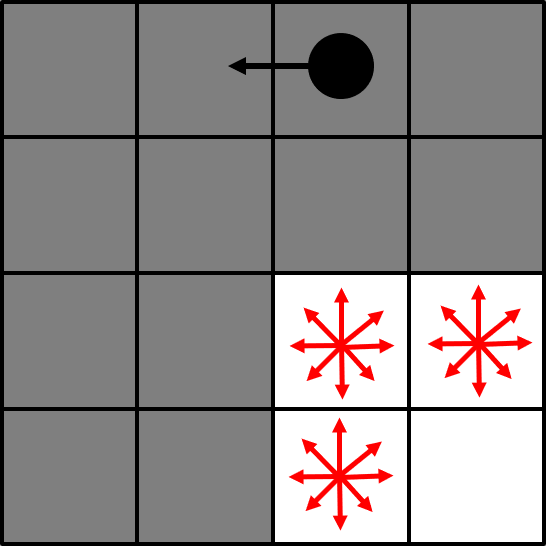
\includegraphics[width=\textwidth]{Report/images/baselinea.png}
        \caption{Candidate configurations}
        \label{subfig:baseline_a}
    \end{subfigure}
    \begin{subfigure}[b]{0.48\textwidth}
        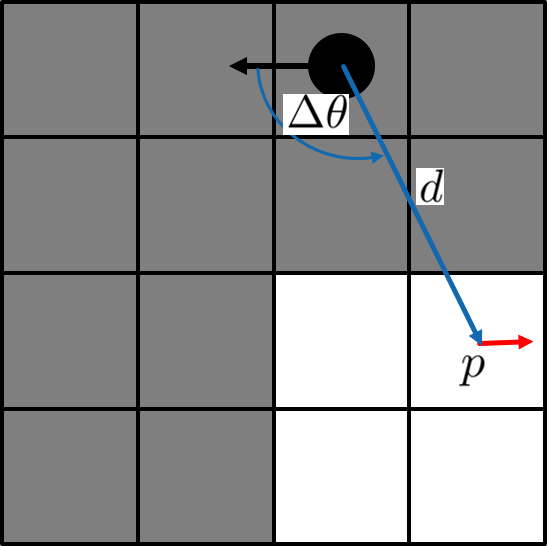
\includegraphics[width=\textwidth]{Report/images/baselineb.png}
        \caption{$\Delta t$ heuristic}
        \label{subfig:baseline_b}
    \end{subfigure}
    \caption{Visualisation of the next-best-view algorithm. The black circle represents the agent's position and the black arrow its orientation. The white cells are unobserved while the dark cells take the value \texttt{observed}. There are three frontier cells shown in (\subref{subfig:baseline_a}). For each frontier cells eight orientations are considered shown with the red arrows. In (\subref{subfig:baseline_b}) the heuristic for constructing $\Delta t$ is depicted.}
    \label{fig:baseline}
\end{figure}

For each candidate configuration $p$ the expected time to transition to $p$ and the expected information gain at $p$ is considered. The expected time $\Delta t$ to transition from the current configuration $p^0$ to $p$ is computed by the heuristic:
%
\begin{equation}
    \Delta t = \frac{\Delta\theta}{\omega_\text{robot}} +    \frac{d}{v_\text{robot}} + \frac{p_\theta - \Delta\theta}{\omega_\text{robot}}
\end{equation}
%
where $v_\text{robot}$ is the agent's speed and $\omega_\text{robot}$ the angular speed. The value $\Delta\theta$ which is depicted in figure \ref{subfig:baseline_b} describes the unsigned angle difference between the current configuration orientation $p_\theta^0$ and the orientation pointing towards the candidate cell and $d$ is the Euclidian distance between $p$ and $p_0$. The expected transition time is encoded in the time-utility $u_{\Delta t}$ as follows:
%
\begin{equation}
    u_{\Delta t} = 1 - \frac{\Delta t - \Delta t_{\text{min}}}{\Delta t_\text{max}-\Delta t_\text{min}}, \quad u_{\Delta_t}\in [0, 1]
\end{equation}
where $\Delta t_\text{min}, \Delta t_\text{max}$ is the minimum respectively the maximum $\Delta t$ value of all the candidate configurations. Note that $u_{\Delta t}$ takes values in range $[0, 1]$, where $1$ corresponds to the closest configuration and $0$ to the furthest.\\

The expected information gain $A$ is given as the expected newly observed area at candidate configuration $p$. It is calculated through simulating the viewing cone of the camera in $p$. Instead of actually computing the area, the \texttt{unobserved} cells within the simulated viewing cone are counted. The area-utility $u_A$ is given by:
\begin{equation}
     u_A = \frac{A-A_{\text{min}}}{A_\text{max}-A_\text{min}}, \quad u_A \in [0, 1]
\end{equation}
where $A_\text{min}, A_\text{max}$ is the minimum respectively the maximum $A$ value of all the candidate configurations. The overall utility of candidate configuration $p$ is given by a weighted average of $u_A$ and $u_{\Delta t}$. The next agent configuration is chosen as the candidate configuration which maximises the overall utility:
%
\begin{equation}
    p_\text{target} = \argmax_{p\in \text{candidates}}\omega_A u_A + \omega_{\Delta t}u_{\Delta t}.
\end{equation}
%

Next-best-view methods are commonly used for exploring unknown environments \cite{5753498, 7487281, Basilico2011}. The method presented does not consider the initial belief distribution over the items nor can it reason which item should be delivered first. The baseline method is therefore not perfectly suited for an object search and delivery task and takes on average longer to complete a delivery than the POMDP agent discussed in the next section.   

%%%%%%%%%%%%%%%%%%%%%%%%%%%%%%%%%%%%%%%%%%%%%%%%%%%%%%%%%%%%%%%%%%%%%%%%%%%%%%%%%%%%%%%%%%%%%%%%%%%%%%%%%%%%%%%%
%%%%%%%%%%%%%%%%%%%%%%%%%%%%%%%%%%%%%%%%%%%%%%%%%%%%%%%%%%%%%%%%%%%%%%%%%%%%%%%%%%%%%%%%%%%%%%%%%%%%%%%%%%%%%%%%
%%%%%%%%%%%%%%%%%%%%%%%%%%%%%%%%%%%%%%%%%%%%%%%%%%%%%%%%%%%%%%%%%%%%%%%%%%%%%%%%%%%%%%%%%%%%%%%%%%%%%%%%%%%%%%%%
\section{POMDP Agent}\label{sec:POMDPagent}

%%%%%%%%%%%%%%%%%%%%%%%%%%%%%%%%%%%%%%%%%%%%%%%%%%%%%%%%%%%%%%%%%%%%%%%%%%%%%%%%%%%%%%%%%%%%%%%%%%%%%%%%%%%%%%%%
\subsection{System Architecture}\label{subsec:sysarch}
\begin{figure}
    \centering
    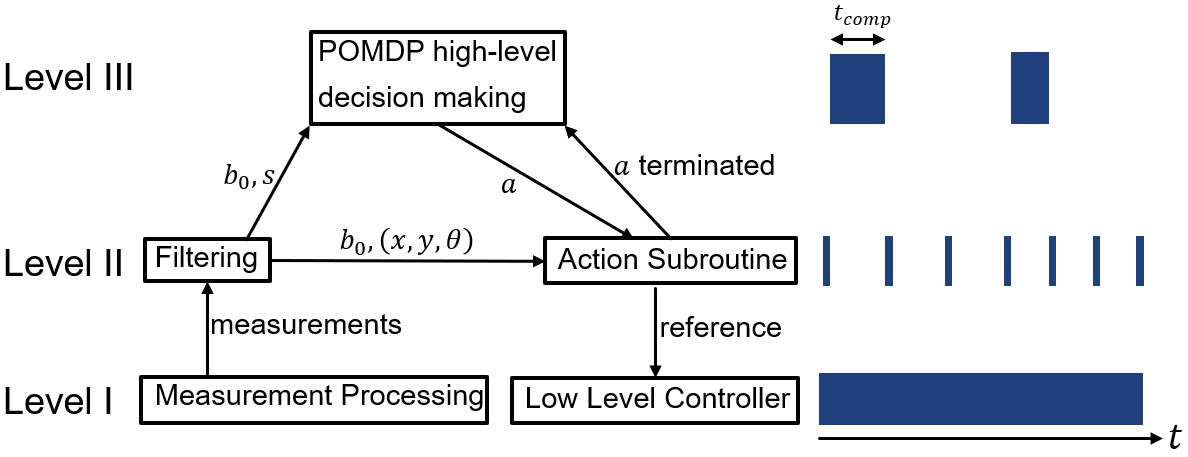
\includegraphics[width=1.0\textwidth]{Report/images/3LevelArchitecture_bothb.png}
    \caption{System Architecture. Level 1 is run at a high frequency. Level 2 updates the reference for the low level controller at regular time intervals. Level 3 is the high-level planner which solves the POMDP with the updated belief when the action subroutine finishes. }
    \label{fig:3levelsarchitecture}
\end{figure}
%
The POMDP model is used for high-level planning in the three level architecture shown in Figure \ref{fig:3levelsarchitecture}. During operation, the lowest level continuously collects measurements, performs state estimation and controls the robot. The measurements are processed at a lower frequency on the second level where the state and belief grid is updated. On the top level is the POMDP solver which computes high-level actions. Each action of the POMDP has a designated execution algorithm henceforth referred to as a \emph{subroutine}. Subroutines belong to the second level of the three layer architecture and are described in more detail in Section \ref{subsec:subroutine}. The subroutine computes a desired reference for the agent and passes it to the lowest level, where it is processed by a feedback controller which moves the robot. Once a subroutine is started the program remains on level 1 and 2 until the subroutine terminates according to its termination criteria. The POMDP on the third level is then solved again using the current belief to produce the next action. This receding horizon procedure is preferred over a precomputed plan, which could fail or result in a suboptimal solution due to model inaccuracies. If the problem should be extended to a dynamic environment, receding horizon control becomes a necessity.\\

The belief grid is an orthogonal high-resolution grid where each cell holds a belief value for each item in the task. Figure \ref{fig:belief_grid} shows the belief grid for the first item in an office environment with three rooms. In Figure \ref{subfig:b_sc03} the initial belief of the problem is shown, where the agent has not make any measurements yet. During operation the belief grid is continuously updated with the camera measurements as shown in Figure \ref{subfig:b_sc03_observed}, where the observed area is colored in violet. Since the item was not observed in those cells the belief that the item is in those locations also drops.\\

%
\begin{figure}[h]
    \centering
    \begin{subfigure}[t]{0.48\textwidth}
        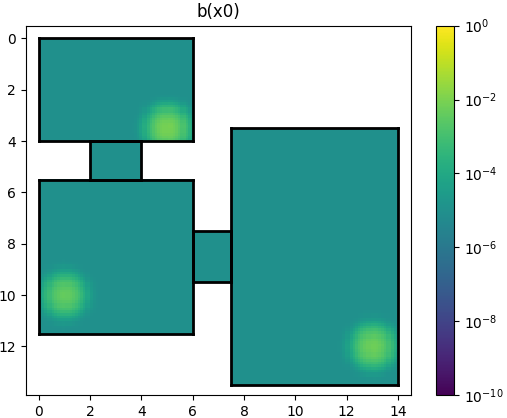
\includegraphics[width=\textwidth]{Report/images/belief_sc03.png}
        \caption{Initial belief grid.}
        \label{subfig:b_sc03}
    \end{subfigure}
    \hfill
    \begin{subfigure}[t]{0.48\textwidth}
        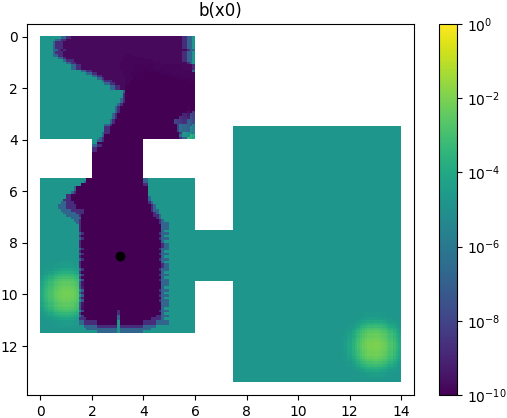
\includegraphics[width=\textwidth]{Report/images/belief_sc03_observed.png}
        \caption{Belief grid after the agent started exploring.}
        \label{subfig:b_sc03_observed}
    \end{subfigure}
    \caption{Belief grid showing the belief of the first item.}
    \label{fig:belief_grid}
\end{figure}
%

The update formula of the belief grid for item $k$ differentiates the case whether the item was observed or not. If the item was observed since the last update the belief value of the cell where the item was spotted is multiplied by the “object recognition rate” $orr<1$, which is the false positive rate of the object recognition algorithm. It takes into account that the classifier could wrongly recognize the item even if it is not present. For all other cells the belief value is multiplied by $1 - orr$. This is to reflect our assumption that there is only one of each item type present in the environment. After all cells are updated, the belief grid is normalized such that the total belief sums to one. The belief values are lower bounded by $10^{-10}$ to avoid numerical rounding issues: 
%
\begin{multline}\label{eq:belief_grid1}
    \texttt{belief\_grid[$k, u, v$]} =\\ 
    \begin{cases} 
        \eta \cdot orr \cdot \texttt{belief\_grid[$k, u, v$]}, &\text{if item $k$ obs. in }c_{(u,v)}; \\
        \eta \cdot \max\left(10^{-10}, (1 - orr) \cdot \texttt{belief\_grid[$k, u, v$]}\right), &\text{otherwise}.
    \end{cases}
\end{multline}
% 
where $c_{(u,v)}$ corresponds to the cell with indices $(u,v)$ and $\eta$ is the normalization factor.\\

If item $k$ was not spotted, the observed cell's belief value is multiplied by $1 - orr_2$, where $orr_2 < 1$ is the false negative rate of the object recognition algorithm. It considers that the classifier could fail to correctly recognize the item if it is present. All other belief values are multiplied by $orr_2$. 
%
\begin{multline}\label{eq:belief_grid2}
    \texttt{belief\_grid[$k, u, v$]} =\\ 
    \begin{cases} 
        \eta \cdot\max\left(10^{-10}, (1 -  orr_2) \cdot \texttt{belief\_grid[$k, u, v$]}\right), &\text{if }c_{(u,v)} \in \mathcal{C}_\text{obs};\\
        \eta \cdot orr_2 \cdot \texttt{belief\_grid[$k, u, v$]}, &\text{otherwise.}
    \end{cases}
\end{multline}
%
where $\mathcal{C}_\text{obs}$ is the set of observed cell since the last belief grid update. Equations \ref{eq:belief_grid1} and \ref{eq:belief_grid2} are motivated by the belief update formula \ref{eq:bdash} where the transition model assumes that the item remains in the same cell and the observation model considers the object recognition algorithm with the variables $orr$ and $orr_2$. 

%%%%%%%%%%%%%%%%%%%%%%%%%%%%%%%%%%%%%%%%%%%%%%%%%%%%%%%%%%%%%%%%%%%%%%%%%%%%%%%%%%%%%%%%%%%%%%%%%%%%%%%%%%%%%%%%
\subsection{POMDP Model}\label{subsec:POMDPmodel}
In this section the POMDP model defined by the tuple $P = \langle \mathcal{S}, \mathcal{A}, \mathcal{O}, T, Z, R, b_0, \gamma \rangle$ is adapted from Van den Hof \cite{Vandenhof} and Mendes \cite{Mendes11} for a search and delivery task involving $m$ items. The environment is divided into $N$ separate non-overlapping regions which from now on are referred to as \textit{nodes}. In figure \ref{subfig:nodes} a small office environment with three rooms is shown which is partitioned into $N=9$ nodes $n_0$ to $n_8$. Nodes can have any shape and do not need to be rectangles.
\begin{figure}
    \centering
    \begin{subfigure}[b]{0.48\textwidth}
        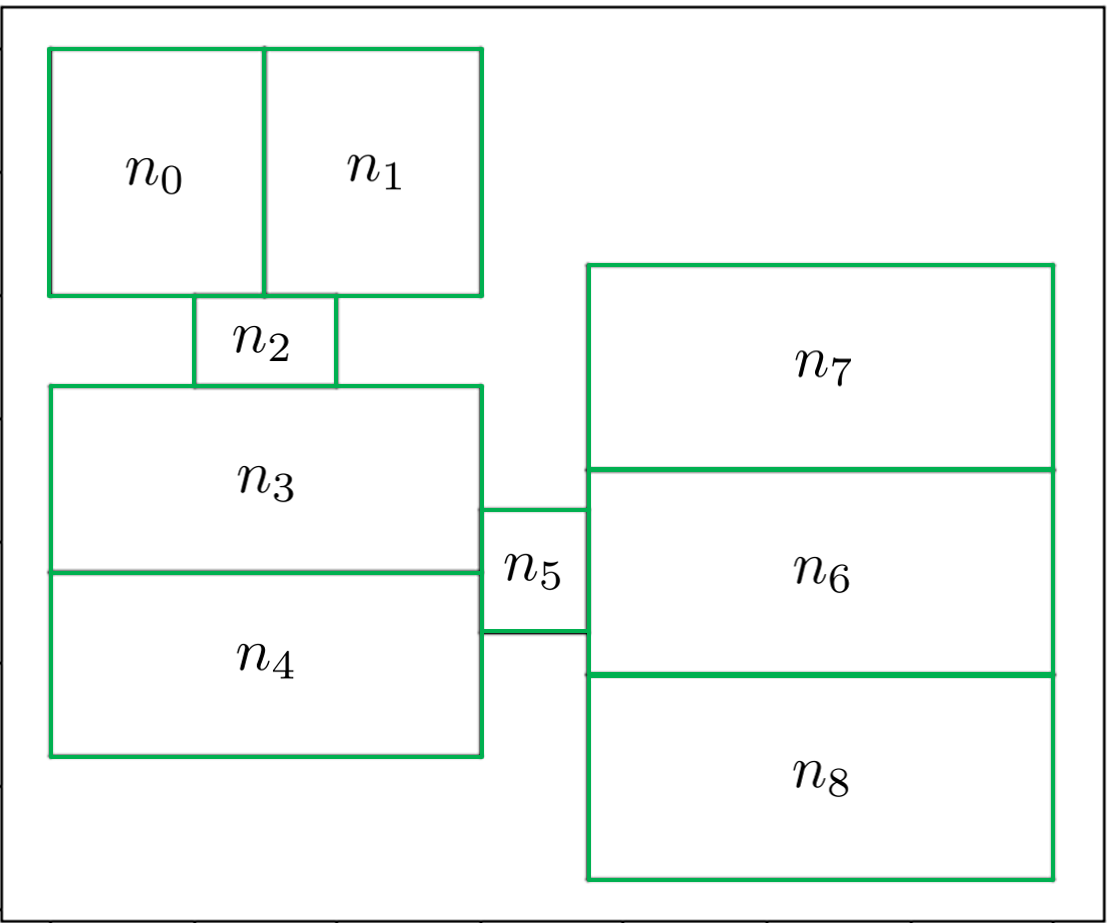
\includegraphics[width=1.0\textwidth]{Report/images/envsmall_l2.png}
        \caption{Node partitioning}
        \label{subfig:nodes}
    \end{subfigure}
    \begin{subfigure}[b]{0.48\textwidth}
    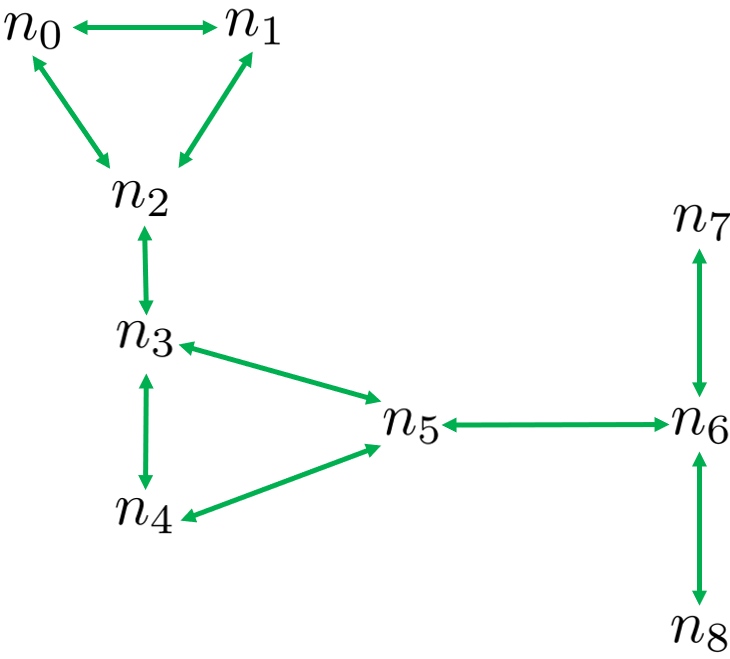
\includegraphics[width=0.9\textwidth]{Report/images/nodeconnectiongraph.png}
        \caption{Connectivity graph}
        \label{subfig:nodeconnection}
    \end{subfigure}
    \caption{A node partitioning of the three room environment and its correspondent connectivity graph.}
    \label{fig:nodes}
\end{figure}
\subsubsection{State Space $\mathcal{S}$}
The state $s$ is represented as a vector of size $K+1$ with one variable describing the agent's position and $K$ variables for the items. The agent's position $x_a$ is specified by the node number and is assumed to be fully observable. This modelling assumption is justified since the area of a node is chosen to take multiple square meters. The item variable $x_k$ of item $k$ is partially observable, as its position is not known beforehand. In addition to the node numbers, $x_k$ takes the values \texttt{agent} when the item is on the agent and the value \texttt{goal} after it is delivered to its goal location:
%%
\begin{equation}
    s=\begin{pmatrix} x_a \\ x_1 \\ \vdots \\ x_K \end{pmatrix}, \qquad \begin{aligned} x_a&\in\{n_0, \cdots, n_N\},\\ 
    x_k &\in \{n_0, \cdots, n_N, \texttt{agent}, \texttt{goal}\}, \quad 1 \leq k \leq K \\
    |\mathcal{S}| &= N(N+2)^K. \end{aligned}
\end{equation}
%%
Since the object search and delivery task has a defined and observable goal, a set of terminal states can be constructed. A state is a terminal state, iff\footnote{if and only if} all item variables take the value \texttt{goal}:
\begin{equation}\label{eq:s_t}
    \mathcal{S}_t = \{s=\begin{pmatrix} x_a & x_1 & \cdots & x_K \end{pmatrix}^\intercal | x_a\in \{n_0, \cdots, n_N\}, x_1=\ldots=x_K=\texttt{goal}\}.
\end{equation}
\subsubsection{Action Space $\mathcal{A}$}
The action space consists of different navigation actions that navigate the agent in between nodes, a \texttt{look\_around} action that aims to observe the node the agent is in, one pickup action for each item and a \texttt{release} action to deliver the item within the current node. A navigation action \texttt{nav($n_i, n_j$)} takes the agent from node $n_i$ to $n_j$ if it currently is in node $n_i$ and vice versa. Navigation actions are only available between two adjacent nodes. See Figure \ref{subfig:nodeconnection} where the node graph of the three-room environment and the navigation actions are visualized. Other choices for navigation actions that require fewer actions in total would be possible. An example for such alternative choice is one navigation action \texttt{nav($n_j$)} per node to navigate the agent from its current node to $n_j$. However, the observation model $Z(o, s', a)$ considers the next state $s'$, not the current state $s$. Clearly, the observation probability of observing an item when choosing a navigation action to node $n_j$ depends on the starting node and the path chosen. With the above choice of navigation action the starting node is implicitly given. Further, by only considering adjacent nodes, the set of possible paths in between the nodes is greatly reduced. This choice of navigation actions therefore allows accurate modelling of the observation function.\\

The \texttt{pickup$k$} action grabs item $k$ in the current node the agent is in. Note that a specific pickup action for each item is required to allow the agent to reason about which item to grab if multiple items are within the same node. Since the agent can only carry one item at a time, one release action suffices. To sum it up, the set of all actions can be written as:
%%
\begin{equation}
    \mathcal{A} = \{\texttt{nav($n_0, n_1$)}, \ldots, \texttt{look\_around}, \texttt{pickup$1$}, \ldots, \texttt{pickup$K$}, \texttt{release}\}.
\end{equation}
%%
\subsubsection{Observation Space $\mathcal{O}$}
The observation $o$ is represented as a vector of size $m$, where each variable corresponds to an item. The observation $o_k$ takes the value \texttt{no} if item $k$ is not observed in this time step, $n_i$ if the item was observed in node $i$ and \texttt{agent} if the agent carries item $k$. If the item variable $x_k$ takes value \texttt{goal} the observation is always \texttt{no}.
\begin{equation}
    o = \begin{pmatrix} o_1 \\ \vdots \\ o_K \end{pmatrix}, \qquad \begin{aligned} o_k &\in \{ \texttt{no}, n_0, \cdots, n_N, \texttt{agent} \}, \quad 1 \leq k \leq K\\
    |\mathcal{O}|&= (N+2)^K \end{aligned}
\end{equation}
\subsubsection{Transition Model $T$}
The transition model $T(s, a, s')$ defines the probability that the agent transitions within one time step to state $s'$ after choosing action $a$ in state $s$. In this model, an entirely deterministic transition model is chosen, i.e., all entries are either one or zero. This implies that given state $s$ and action $a$, the next state $s'$ is known. Further, conditional independence between the state variables of the next state $s'$ given action $a$ and the current state $s$ is assumed. The transition function can therefore be calculated by multiplying the transition model for each state variable:
%%
\begin{equation}
    \left(x_a' \upmodels x_1' \upmodels \cdots \upmodels x_K' |a, s\right) \Rightarrow T(s,a,s') = T(s,a, x_a') T(s,a,x_1') \cdots T(s,a,x_K').
\end{equation}
%%
This assumption reduces the number of entries in the transition model from \\$\left(N(N+2)^K\right)^2\cdot|\mathcal{A}|$ to $N(N+2)^K\cdot|\mathcal{A}|\cdot (N+K(N+2))$. The transition function $T(s, a, x_a')$ is stated in Equations \ref{eq:Tnavxa} - \ref{eq:Tstxa}. Equation \ref{eq:Tnavxa} formalizes that the agent transitions from position $x_a=n_i$ to node $n_j$ and vice versa if the corresponding navigation action \texttt{nav($n_i,n_j$)} is chosen:
%%
\begin{equation}\label{eq:Tnavxa}
    T(s, a=\texttt{nav($n_i, n_j$)}, x_a') = \begin{cases}
             1, & \text{if }x_a=n_i \land x_a'=n_j;\\
             1, & \text{if }x_a=n_j \land x_a'=n_i;\\
             0, & \text{otherwise}.
         \end{cases}
\end{equation}
%%
For the actions \texttt{look\_around}, \texttt{release} and pickup actions the agent remains in the same node: 
%%
\begin{equation}
    T(s,a\in\{\texttt{look\_around}, \texttt{pickup}1,\cdots,\texttt{pickup}K, \texttt{release}\}, x_a') = 
    \begin{cases}
        1, & \text{if }x_a=x_a'; \\
        0, & \text{otherwise}.
    \end{cases}
\end{equation}
%%
Finally, if the current state is a terminal state $s_t$, the agent remains per definition in that terminal state:
%%
\begin{equation}\label{eq:Tstxa}
    T(s\in\mathcal{S}_t, a, x_a') = \begin{cases}1, &\texttt{if }x_a'=x_a;\\
         0,& \texttt{otherwise}.\end{cases}
\end{equation}
%%
The transition function $T(s, a, x_k')$ for item $k$ is defined in Equations \ref{eq:Txkremain} - \ref{eq:Txkts}. For navigation actions and the \texttt{look\_around} action the items remain in the same state. The navigation action only affects variable $x_a$. If the agent is carrying item $k$, the item takes value \texttt{agent} and is unaffected by navigating. The \texttt{look\_around} action is used to search the current node for items, but does not directly affect the item's location:    
%%
\begin{equation}\label{eq:Txkremain}
    T(s, a=\in\{\texttt{nav($n_i, n_j$)},\texttt{look\_around}\}, x_k') = \begin{cases}
             1, & \text{if }x_k'=x_k;\\
             0, & \text{otherwise}.
         \end{cases}
\end{equation}
%%
If the agent selects the \texttt{pickup} action the item transitions to state \texttt{agent}, given that the agent is not carrying another item and is in the same node as the item. Otherwise, the item remains in the same state. Note that a deterministic pickup model is a simplification, as the pickup-subroutine (see subsection \ref{subsec:subroutine}) can fail even if $x_a=x_k$ as it's not guaranteed that the agent observes the item.
%%
\begin{equation}\label{eq:Txkpickup}
T(s,a=\texttt{pickup}k, x_k') = \begin{cases}
             1, & \text{if }x_a=x_k \land x_e\neq \texttt{agent} \land x_k'=\texttt{agent}, 1\leq e\leq K, e\neq k;  \\
             1, & \text{if }x_a \neq x_k \land x_k=x_k'; \\
             0, & \text{otherwise.}
         \end{cases}
\end{equation}
%%
Equation \ref{eq:Txkrelease} shows the transition model for the \texttt{release} action. If the agent is carrying item $k$ and is in the node where the goal location $g_k$ of item $k$ is located, then the item is successfully delivered within this time step and takes value $\texttt{goal}$. If the release action is chosen in a different node the item is dropped at the agent's current location and therefore takes a node value. An item is not affected by the \texttt{release} action if the agent is not carrying it:
%%
\begin{equation}\label{eq:Txkrelease}
    T(s,a=\texttt{release}, x_k') = \begin{cases}
             1, & \text{if }x_k =\texttt{agent} \land x_a = g_k \land x_k' = \texttt{goal}; \\
             1, & \text{if }x_k =\texttt{agent} \land x_a \neq g_k \land x_a = x_k'; \\
             1, & \text{if }x_k\neq \texttt{agent} \land x_k'=x_k; \\
             0, & \text{otherwise}. 
             \end{cases}
\end{equation}
%%
Item $k$ is not allowed to change value if the current state is a terminal state:
%%
\begin{equation}\label{eq:Txkts}
    T(s\in\mathcal{S}_t, a, x_k') = \begin{cases}1, &\texttt{if }x_k=x_k';\\
         0,& \text{otherwise}.\end{cases}
\end{equation}
%%
\subsubsection{Observation Model $Z$}
The observation model $Z(o, s', a)$ defines the probability of receiving observation $o$ given that the time step ends in state $s'$ after choosing action $a$. In this model conditional independence between the observation variables $o_k$ is assumed, given $s'$ and $a$. This assumption does not always hold, as some items are often co-located. For example the items salt and pepper are often located next to each other.  If the probability of observing the salt is high it is likely that the pepper is observed too. However, the assumption simplifies the design process as it allows writing the observation function $Z(o, s', a)$ as product of the individual observation functions $Z(o_k, s', a)$:
%%
\begin{equation}\label{eq:Ocondind}
    \left(o_1 \upmodels \cdots \upmodels o_K |s', a\right) \Rightarrow Z(o,s',a) = \prod_{1\leq k \leq K}Z(o_k,s',a).
\end{equation}
%%
Equations \ref{eq:Onav} - \ref{eq:Orelease} show the observation function for item $k$. The probability of observing the item during a navigation action in node $n_q$ is approximated as the ratio between the expected observed area of node $n_q$ and the total area of node $n_q$. See Figure \ref{fig:obsmodel} for a visualization of the expected observed area. The ratio gets multiplied by the constant $orr_2$ (see Equation \ref{eq:belief_grid2}). This model does not consider which part of the area of the node is observed. If the agent were to execute the same navigation action a second time with the same starting end ending node, the observed area will be the same as in the first navigation action. The agent however would expect the initial probability of observing an item. This model inaccuracy could in the worst case lead to the agent driving back and forth between the same nodes in an attempt to observe the nodes. Since the algorithm is run in a receding horizon fashion, this inaccuracy can be corrected for by reducing the observation probability for a navigation action if it was chosen in previous time steps.\\

The probability of not observing the item even though it is present in node $n_q$ is given by one minus the probability of observing the item. If the agent carries the item after the action finished, the observation is always $\texttt{agent}$ independent of which action was chosen. Since an item that already got delivered must no longer be considered the observation of that item is assumed to be \texttt{no}. All other cases, for example that the object recognition algorithm wrongly observes an item in a node where it is not present are neglected and set to zero probability: 
%%
\begin{equation}\label{eq:Onav}
    Z(o_k, s', a=\texttt{nav($n_i, n_j$)}) = 
    \begin{cases}
        orr_2 \cdot \frac{\text{observed area of }n_q}{\text{area of }n_q}, & \text{if }o_k=x_k'=n_q ;\\
        1 - orr_2 \cdot \frac{\text{observed area of }n_q}{\text{area of }n_q}, & \text{if } o_k=\texttt{no}\land x_k'=n_q;\\
        1, & \text{if }o_k=x_k'=\texttt{agent};\\
        1, & \text{if }o_k=\texttt{no}\land x_k'=\texttt{goal};\\
        0, & \text{otherwise}.
    \end{cases}
\end{equation}
\begin{figure}
    \centering
    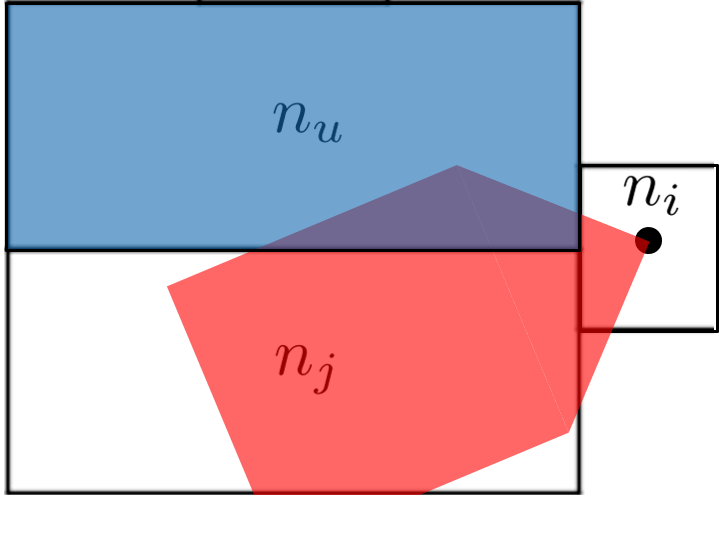
\includegraphics[width=0.5\textwidth]{Report/images/observationmodel.png}
    \caption{Visualization of the observation model for the navigation action. The red area shows the expected observed area of action $a=\texttt{nav($n_i, n_j$)}$.}
    \label{fig:obsmodel}
\end{figure}
%%
For the \texttt{look\_around} action the probability of observing the item in the current node is chosen as ninety percent. Consequently the probability of not observing the item is set to ten percent. The fact that the item could be observed in a different node than the one the agent is currently examining is neglected:
%%
\begin{equation}\label{eq:lookaround}
    Z(o_k, s', a=\texttt{look\_around}) = \begin{cases}
    0.9,& \text{if } o_k=x_a'=x_k';\\
    0.1, &\text{if } o_k=\texttt{no} \land x_a'=x_k';\\
    1,& \text{if }o_k=x_k'=\texttt{agent};\\
    1,& \text{if }o_k=\texttt{no}\land x_a'\neq x_k';
    \\0, &\text{otherwise}. \end{cases}
\end{equation}
%%
A pickup action is assumed to succeed if the agent observes the item in the current node and to fail otherwise. The probability of observing \texttt{no} is therefore one if the agent is not carrying the item after the action is finished. If the action succeeds the item is on the agent and the observation is \texttt{agent}:
%%
\begin{equation}\label{eq:pickup}
    Z(o_k, s', a=\texttt{pickup}k) = \begin{cases}
    1, &\text{if } o_k=\texttt{no} \land x_k'\neq \texttt{agent};\\
    1,& \text{if }o_k=x_k'=\texttt{agent};\\
    0, &\text{otherwise}. \end{cases}
\end{equation}
%%
If the agent carries item $k$ and selects the release action, then the next item state is known. No informative observation is needed. Therefore the probability of observing \texttt{no} is set to one. The probability of observing a different item during releasing item $k$ is neglected. This simplification is well justified, since releasing an item for the sake of observing a different item is most likely not a time-efficient behaviour. Similarly, the probability of observing item $k$ during the pickup action of item $e$ where $k\neq e$ is assumed to be zero. 
%%
\begin{equation}\label{eq:Orelease}
    Z(o_k, s', a\in\{\text{pickup}e, \texttt{release}\}) = \begin{cases}
    1,& \text{if } o_k=\texttt{no};\\
    0,& \text{otherwise}.\end{cases}
\end{equation}
%%
\subsubsection{Reward Model $R$}
Reward models are used to capture the objectives of the task the agent should solve. The goal of this object search and delivery problem is to find the items and deliver them to their target locations in as little time as possible. The reward function used for this task can be split into a time penalty $R_\text{time}$, a reward  $R_\text{subtask}$ for picking an item up and a reward $R_\text{task}$ for delivering an item to its target location. The time penalty makes sure that the optimal policy of the POMDP minimizes the expected completion time of the deliveries. The subtask and task rewards guide the POMDP solver towards the terminal state and thus leads to faster convergence:
%%
\begin{equation}
    R = R_{\text{time}} + R_{\text{subtask}} + R_{\text{task}}.
\end{equation}
%%
Execution times of the actions in the POMDP differ and are not previously known, since they are high-level actions that are processed by their designated subroutine. The run-time of the subroutines depend on the specific agent location, item positions and the current state of the belief grid. Modelling $R_\text{time}$ requires approximating these execution times, either through a simulation using sampling to get robust averaged values or by using a heuristic. In the implementation of this model the simulation approach was used.\\
The expected run-time of the navigation function is given by $t_\texttt{nav}(n_i, n_j)$ where $n_i$ is the start node and $n_j$ the target node. To avoid that the agent picks a navigation action that is not available in the its current position, a high negative reward is given for unavailable navigation actions
\begin{equation}
    R_\text{time}(s, a=\texttt{nav($n_i, n_j$)}) = \begin{cases}
    -t_\texttt{nav}(n_i, n_j), & \text{if } x_a=n_i;\\
    -t_\texttt{nav}(n_j, n_i), & \text{if } x_a=n_j;\\
    -1000 & \text{otherwise}.
    \end{cases}
\end{equation}
The expected time $t_\texttt{l\_a}$ of the \texttt{look\_around} action is node-dependent since nodes have different shapes and sizes. Further, $t_\texttt{l\_a}$ differs depending on if an item is present or not as is explained in subsection \ref{subsec:subroutine}. 
%%
\begin{multline}
    R_\text{time}(s, a=\texttt{look\_around}) = \\\begin{cases}
    -t_\texttt{l\_a}(n_i, \texttt{item\_present=True}), & \text{if }x_a=n_i \land x_k=n_i, \quad 1\leq k \leq K;\\
    -t_\texttt{l\_a}(n_i, \texttt{item\_present=False}), & \text{if }x_a=n_i \land x_k \neq n_i,\quad  1\leq k \leq K.
    \end{cases}
\end{multline}
%%
For the pickup action  the same considerations as for the \texttt{look\_around} action are made. The time penalty $R_\text{time}$ is given by:
\begin{multline}
    R_\text{time}(s, a=\texttt{pickup}k) = \\ \begin{cases}
    -t_\texttt{pickup}(n_i, \texttt{item\_present=True}), & \text{if }x_a=n_i \land x_k=n_i, \quad 1\leq k \leq K;\\
    -t_\texttt{pickup}(n_i, \texttt{item\_present=False}), & \text{if }x_a=n_i \land x_k \neq n_i,\quad  1\leq k \leq K.
    \end{cases}
\end{multline}
%%
% Note that the choice of $t_\texttt{pickup}(n_i, \texttt{item\_present=False})$ can be critical for a good performance. Ideally, the agent chooses the \texttt{look\_around} action if it isn't sure if the item is present. If the item is then observed a pickup action with expected time $t_\texttt{pickup}(n_i, \texttt{item\_present=True})$ should be chosen. If $t_\texttt{pickup}(n_i, \texttt{item\_present=False})$ is chosen too low, the agent will always choose the pickup action instead of the \texttt{look\_around} action, which yields bad performance as the pickup subroutine is not made for exploration. 


% \begin{multline}
% t_\texttt{pickup}(n_i, \texttt{item\_present=False}) > \\
%     t_\texttt{l.a}(n_i, \texttt{item\_present=False}) + t_\texttt{l.a}(n_i, \texttt{item\_present=True})
% \end{multline}

Finally, for the release action the expected execution time differs depending on whether the agent is in the item's goal node $g_k$ or not. In the goal node the agent first has to drive to the goal coordinates, while in any other node the item is dropped at the agent's current location: 
%%
\begin{equation}
     R_\text{time}(s, a=\texttt{release}) = \begin{cases}
    -t_\texttt{release\_goal}(n_i), & \text{if }x_a=g_k \land x_k=\texttt{agent}, \quad 1 \leq k \leq K; \\
    -t_\texttt{release\_drop}(n_i), & \text{if }x_a\neq g_k \land x_k=\texttt{agent}, \quad 1 \leq k \leq K;\\
    0, & \text{if }x_k \neq \texttt{agent}, \quad 1 \leq k \leq K.
    \end{cases}
\end{equation}
%%
The agent receives a positive reward $r_\text{pickup}$ for successfully grabbing an item. When the agent releases the item in a later time step the same reward must be subtracted. Without the negative reward for releasing an item, the agent would repeatedly pick an item up and release it right afterwards to gather the subtask reward. Note that $R_\text{subtask}(s,a,s')$ is written as a function of the current state $s$, action $a$ and the next state $s'$. Indeed, all the equations in Chapter \ref{chap:probabilistic} can be adapted without further adjustments to a reward model that is a function of $s'$ as well. 
 %%
\begin{equation}
    R_\text{subtask}(s,a,s') = \begin{cases}
    +r_\text{pickup}, & \text{if }a=\texttt{pickup}k \land x_k'=\texttt{agent};\\
    -r_\text{pickup}, & \text{if }a=\texttt{release}\land x_k=\texttt{agent};\\
    0, & \text{otherwise}.\end{cases}
\end{equation}
%%
Similarly, there is a positive reward $r_\text{delivery}$ for delivering an item to its goal location. The transition model does not allow the agent to pick an item up if it takes the value \texttt{goal}, therefore no negative reward for that case is required. 
%%
\begin{equation}
    R_\text{task}(s,a,s') = \begin{cases} + r_\text{delivery}, & \text{if }a=\texttt{release}\land x_k'=\texttt{goal}\land x_k=\texttt{agent};\\
    0, & \text{otherwise}.
    \end{cases}
\end{equation}
%%
\subsubsection{Initial Belief $b_0$}
The initial belief $b_0(s)$ is a distribution that defines the probability for each value of the partially observable variables in state $s$. Since the belief grid (see subsection \ref{subsec:sysarch}) considers the items independent of each other, the belief can be expressed as a product of the belief $b_0(x_k)$ of each item:
\begin{equation}\label{eq:b0_prod}
    b_0(s) = \prod_{1\leq k\leq K} b_0(x_k).
\end{equation}

In Equation \ref{eq:b0_prod} the belief $b_0$ represents a distribution. The belief $b_0(x_k)$ of item $k$ can also be represented as a vector where each element corresponds to a probability of an item value:
\begin{equation}
    b_0(x_k) = \begin{pmatrix} b_0(x_k=n_0) & \cdots & b_0(x_k=n_N) & b_0(x_k=\texttt{agent}) & b_0(x_k=\texttt{goal}) \end{pmatrix}^\intercal.
\end{equation}
%%
To calculate the probability that the item is in node $n_i$, the cells $\mathcal{C}(n_i)$ of the belief grid that lie within $n_i$ are aggregated:
%%
\begin{equation}
b_0\left(x_k=n_i\right) = \sum_{c_{(u,v)}\in \mathcal{C}(n_i)}\texttt{belief\_grid[$k, u, v$]}.
\end{equation}
%%
Note that item value \texttt{agent} and \texttt{goal} are observable values and the initial belief is therefore either one if the item is on the agent or already delivered and zero otherwise. 
%%
\subsubsection{Discount Factor $\gamma$}
Discounting can be used to value future rewards less than current ones and is required for some solving methods like Sarsop (see subsection \ref{subsec:SARSOP}). Since the goal of this object search and delivery problem is to minimize the total time, the discounting factor is chosen close to one:
\begin{equation}
    \gamma = 0.999.
\end{equation}
%%
%%%%%%%%%%%%%%%%%%%%%%%%%%%%%%%%%%%%%%%%%%%%%%%%%%%%%%%%%%%%%%%%%%%%%%%%%%%%%%%%%%%%%%%%%%%%%%%%%%%%%%%%%%%%%%%%
\subsection{Subroutines}\label{subsec:subroutine}
After the POMDP solver selects an action the designated subroutine takes over and creates the reference for the robot controller. Each subroutine has termination criteria that determine the end of the action, after which the POMDP is resolved. Only one criteria needs to be fulfilled for termination. There is one subroutine for all navigation actions, one for all pickup actions, one for the \texttt{release} action and one for the \texttt{look\_around} action. A possible implementation of each subroutine is briefly outlined below.\\

To steer the agent between two nodes, the navigation subroutine of action \texttt{nav($n_i, n_j$)} computes the shortest path to the mid-point of node $n_j$ for starting node $n_i$ and vice versa. All subroutines use the $A^*$-algorithm for path planning. The action is terminated as soon as the agent is in the target node or if there is a sudden increase in the belief grid, which means that an item was detected. The criteria for the belief increase requires a cell with belief higher than $0.9$ and an increase in belief since the start of the subroutine of at least $1.05$. The exact choice of those tuning parameters does not matter too much. \\

\textit{Termination criteria for the navigation subroutine:}
\begin{align}
    \text{criteria 1}&: \quad
    \begin{cases}x_a == n_j, &\text{if the agent started in }n_i;\\ 
    x_a == n_i, & \text{if the agent started in }n_j. \end{cases}\\
    \text{criteria 2}&:\quad \frac{\texttt{b\_max}}{\texttt{b\_max\_0}} > \max\left(1.05, \frac{0.9}{\texttt{b\_max\_0}}\right)\label{eq:subr_crit2}
\end{align}

where \texttt{b\_max\_0} is the maximum belief value of the belief grid at the start-time of the subroutine and \texttt{b\_max} is the current maximum belief value. \\

The pickup subroutine aims at grasping the item in the current node and assumes that the item does not need to be searched for first. For action $\texttt{pickup}k$ the subroutine sets the path to the belief cell with the highest belief value of item $k$. During execution the belief grid is continuously updated and the target cell adapted to the one with maximum belief. If the target cell is reached, the agent grabs the item and the subroutine terminates. If another, previously unobserved item is discovered during execution, the subroutine terminates, as the optimal action to execute might be a different one now. To avoid that the agent drives around the node forever, which would be the case if the item is not present, the action terminates if the total belief of item $k$ within the current node drops below a threshold.\\

\textit{Termination criteria for the pickup subroutine:}
\begin{align}
    \text{criteria 1}&: \quad x_k == \texttt{agent}\\
    \text{criteria 2}&: \quad \frac{\texttt{b\_max}}{\texttt{b\_max\_0}} > \max\left(1.05, \frac{0.9}{\texttt{b\_max\_0}}\right)\\
    \text{criteria 3}&: \quad \frac{\texttt{b\_tot}}{\texttt{b\_tot\_0}} < 0.25
\end{align}

where \texttt{b\_max} and \texttt{b\_max\_0} are the max belief value of any item $u\neq k$, \texttt{b\_tot\_0} is the aggregated belief of item $k$ in the current node at the start time of the subroutine and \texttt{b\_max} the current aggregated belief.\\

The purpose of the \texttt{look\_around} subroutine is to discover items in the current node. A next-best-view method similar to the baseline method (Section \ref{sec:baseline}) can be used for this search task. The utilities are $u_{\Delta t}$ which corresponds to the expected time to transfer to the target pose $p$ and $u_b$  which considers the summed belief the agent expects to observe at $p$:
\begin{equation}
    p_\text{target} = \argmax_{p\in \text{candidates}} \left(\omega_{\Delta t}u_{\Delta t}(p)+ \omega_b u_b(p)\right)
\end{equation}
where $\omega_{\Delta t}$ and $\omega_b$ are scalar weights and the candidate configurations are determined as the frontier cells plus eight orientations, analogously to the baseline agent. A new target pose is chosen once the current is reached. The subroutine terminates if more than ninety per cent of the node area was observed since the subroutine started, which corresponds to the specified observation probability of the observation model. It also terminates if the maximum belief increased, which indicates that an item was discovered or if the belief peak of the node is reduced strongly enough. The later considers the difference between the highest belief values and the median belief value of the current node and its change since the start of the action. \\

\textit{Termination criteria for the \texttt{look\_around} action:}
\begin{align}
    \text{criteria 1}&: \quad \frac{\text{observed area of current node}}{\text{unobserved area of current node}} > 0.9\\
    \text{criteria 2}&: \quad \frac{\texttt{b\_max}}{\texttt{b\_max\_0}} > \max\left(1.05, \frac{0.9}{\texttt{b\_max\_0}}\right)\\
    \text{criteria 3}&: \quad  \texttt{b\_max\_N} - \texttt{b\_m} < \frac{1}{20}\cdot (\texttt{b\_max\_N\_0} - \texttt{b\_m\_0})
\end{align}
where \texttt{b\_m} is the median belief value of the current node, \texttt{b\_max\_N} is the averaged belief of the $N$ maximum belief values and \texttt{b\_max\_N\_0}, \texttt{b\_m\_0} are the same values at start time. It is of course possible that the \texttt{look\_around} subroutine does not find the item even if it is present. The agent can select the same action again if it still beliefs that the item is there.\\

The behaviour of the release subroutine depends on the current node the agent is in. If the goal location of the carried item is within the current node, the subroutine sets the shortest path to the goal location as reference and then releases the item. Otherwise, the item is just released at the agent's current location. The action finishes as soon as the item is not on the agent anymore.
%%%%%%%%%%%%%%%%%%%%%%%%%%%%%%%%%%%%%%%%%%%%%%%%%%%%%%%%%%%%%%%%%%%%%%%%%%%%%%%%%%%%%%%%%%%%%%%%%%%%%%%%%%%%%%%%
\subsection{Model Extensions}\label{subsec:POMDP_extensions}
This subsection looks at the assumptions made in the problem definition (section \ref{sec:problemdef}) and how they can be loosened by adapting the above presented POMDP problem. \\

One of the most unrealistic assumptions is the absence of furniture. In most offices mugs do not lie on the floor but are in a cupboard, in the dishwasher or on a table. Furniture can be added to the POMDP model by handling it as a node. The \texttt{look\_around} and pickup subroutine would need to be adapted to be able to interact with it. Further, the observation probability for navigating to the furniture needs to be adapted. For a cupboard the probability of observing the mug while approaching the cupboard should be zero assuming that the cupboard is closed while the mug could be spotted if it is on a table.\\

A real office does not satisfy the assumption of a static environment as there are moving obstacles and people interacting with the searched items. 
The solution framework presented in this section can be used for such environments without further adaptions on the POMDP model, as it is used as a high-level planner. The subroutines need to be generalised with moving obstacle avoidance and more flexible termination criteria. A mean employee could for example steal the item the robot is currently carrying. In such a case the agent should immediately stop the current subroutine and re-solve the POMDP. Further, the update formula for the belief grid could be adapted to the dynamic environment. Consider the task where the agent should find the milk. As the milk is usually in the refrigerator the agent would check there. However, the milk might not be there as the previous refrigerator user forgot to put it back. As the milk was not observed the belief that the milk is in the refrigerator decreases. The agent will not check the fridge for a long time as the execution time of opening and closing the fridge yields a large time penalty $R_\text{time}$ and the belief of the milk being there is small. In reality it is very likely that another coworker sees the milk and puts it back in the fridge. The belief update formula can be adapted such that the belief goes back to the initial belief as time passes. In particular, Equation \ref{eq:belief_grid2} for the case where item $k$ was not observed should be changed to:
\begin{multline}
    \texttt{bg[$k, u, v$]} = \\
    \begin{cases} 
        \eta \cdot\max\left(10^{-10}, (1 -  orr_2) \cdot \texttt{bg[$k, u, v$]}\right), &\text{if }c_{(u,v)} \in \mathcal{C}_\text{obs};\\
        \eta \cdot \max\left(10^{-10}, orr_2 \cdot \sum_{(p,q)}p(c_{(u,v)}|c_{(p,q)}) \cdot \texttt{bg[$k, p, q$]}\right), &\text{otherwise}.
    \end{cases}
\end{multline}
where \texttt{bg} is the belief grid and $p(c_{(u,v)}|c_{(p,q)})$ can be interpreted as the probability that the item transitions from cell $(p,q)$ to cell $(u,v)$. This probability can be expressed such that the belief of $c_{(u,v)}$ goes back to its initial belief: 
\begin{equation}
    p(c_{(u,v)}|c_{(p,q)}) = \begin{cases}
    \epsilon \cdot \texttt{bg\_0[$k, u, v$]}, &\text{if } (u,v)\neq (p,q);\\
    1 - \epsilon \cdot (1-\texttt{bg\_0[$k, u, v$]}), &\text{otherwise}.
    \end{cases}
\end{equation}
where $\epsilon$ is a constant that determines how fast the initial belief is reached.\\

The simplification that only one item of each type is present is restrictive for a service robot. A task might involve delivering two mugs in an environment with many mugs and the user does not care which specific mug is delivered. To loosen this assumption, the belief grid normalization procedure needs to be adapted such that the summation over the entire belief grid is equal to the number of mugs in the environment. The update equations for the belief grid (equations \ref{eq:belief_grid1} and \ref{eq:belief_grid2}) need to be changed. They are based on the assumption that the item can only be at one place at a time, which is not the case in an environment with multiple indistinguishable items.
 
%%%%%%%%%%%%%%%%%%%%%%%%%%%%%%%%%%%%%%%%%%%%%%%%%%%%%%%%%%%%%%%%%%%%%%%%%%%%%%%%%%%%%%%%%%%%%%%%%%%%%%%%%%%%%%%%
%%%%%%%%%%%%%%%%%%%%%%%%%%%%%%%%%%%%%%%%%%%%%%%%%%%%%%%%%%%%%%%%%%%%%%%%%%%%%%%%%%%%%%%%%%%%%%%%%%%%%%%%%%%%%%%%
%%%%%%%%%%%%%%%%%%%%%%%%%%%%%%%%%%%%%%%%%%%%%%%%%%%%%%%%%%%%%%%%%%%%%%%%%%%%%%%%%%%%%%%%%%%%%%%%%%%%%%%%%%%%%%%%
\section{Multi-Scale POMDP Agents}\label{sec:Multi-Scale}
POMDPs are computationally intractable to solve for large problems. As is shown later in Chapter \ref{sec:results} the POMDP agent scales poorly with increasing problem size and is unsuitable for a one item task in a large office environment. In this section a novel hierarchical POMDP framework is presented which greatly reduces computation times. The original POMDP problem is split into multiple smaller problems with different spatial resolutions. First the top layer with a coarse resolution is solved and its proposed action is then refined. The lowest layer of the hierarchy corresponds to the original POMDP problem.\\

In Section \ref{subsec:Multi-Scale_overview} the hierarchical framework is explained and in section \ref{sec:M1toM3} three different methods to combine the spatial layers are presented. Section \ref{subsec:Multi-Scale_properties} discusses properties of the Multi-Scale methods regarding solution quality and scaling. 

%%%%%%%%%%%%%%%%%%%%%%%%%%%%%%%%%%%%%%%%%%%%%%%%%%%%%%%%%%%%%%%%%%%%%%%%%%%%%%%%%%%%%%%%%%%%%%%%%%%%%%%%%%%%%%%%
\subsection{Overview} \label{subsec:Multi-Scale_overview}
Multi-Scale methods first solve the top layer $l0$ which yields the value function $V(b^{l0})$ and the first action to execute $a^{l0}$. The superscript $l\lambda$ indicates that the variable belongs to layer $\lambda$. Next, layer 1 is solved and afterwards layer 2 and so on. On the lower layers only a subset of the state, observation and action space is considered, determined by the action and state of the layer above. The Multi-Scale methods presented do not compute the entire solution beforehand but only the next action to execute. In the following the hierarchical layout is shown in more detail and then the higher layer transition, reward and observation models are derived.
%%%%%%%%%%%%%%%%

\subsubsection{Hierarchical Layout}
The Multi-Scale POMDP arranges the environment into multiple layers with different levels of discretisation. In Figure \ref{fig:two_layers} the three room environment is shown with two spatial layers. Each node of layer 1 can be mapped to only one node of layer 0. The node layout is chosen manually for the examples of this thesis. 
\begin{figure}
    \centering
    \begin{subfigure}[b]{0.48\textwidth}
        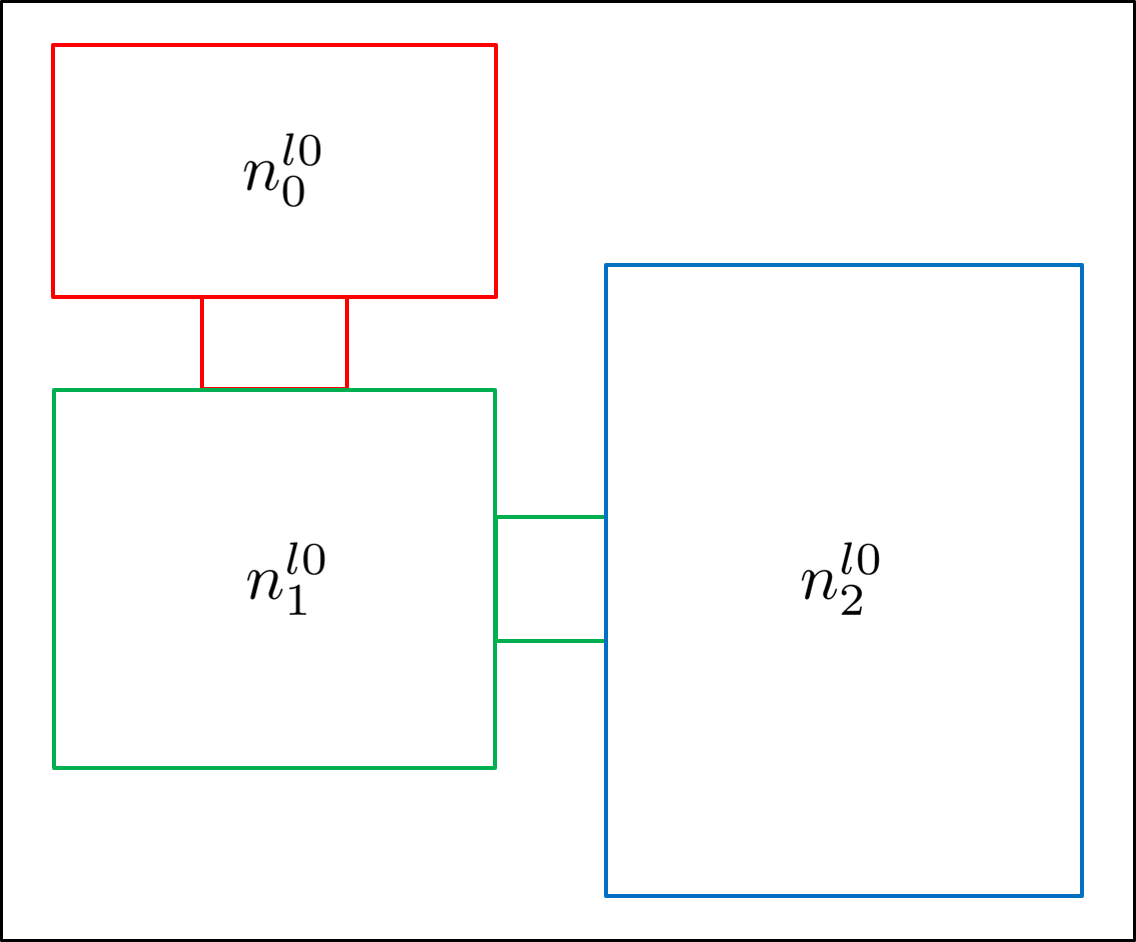
\includegraphics[width=\textwidth]{Report/images/layer0_b.png}
        \caption[t]{Layer 0}
        \label{subfig:l0}
    \end{subfigure}
    \hfill
    \begin{subfigure}[b]{0.48\textwidth}
        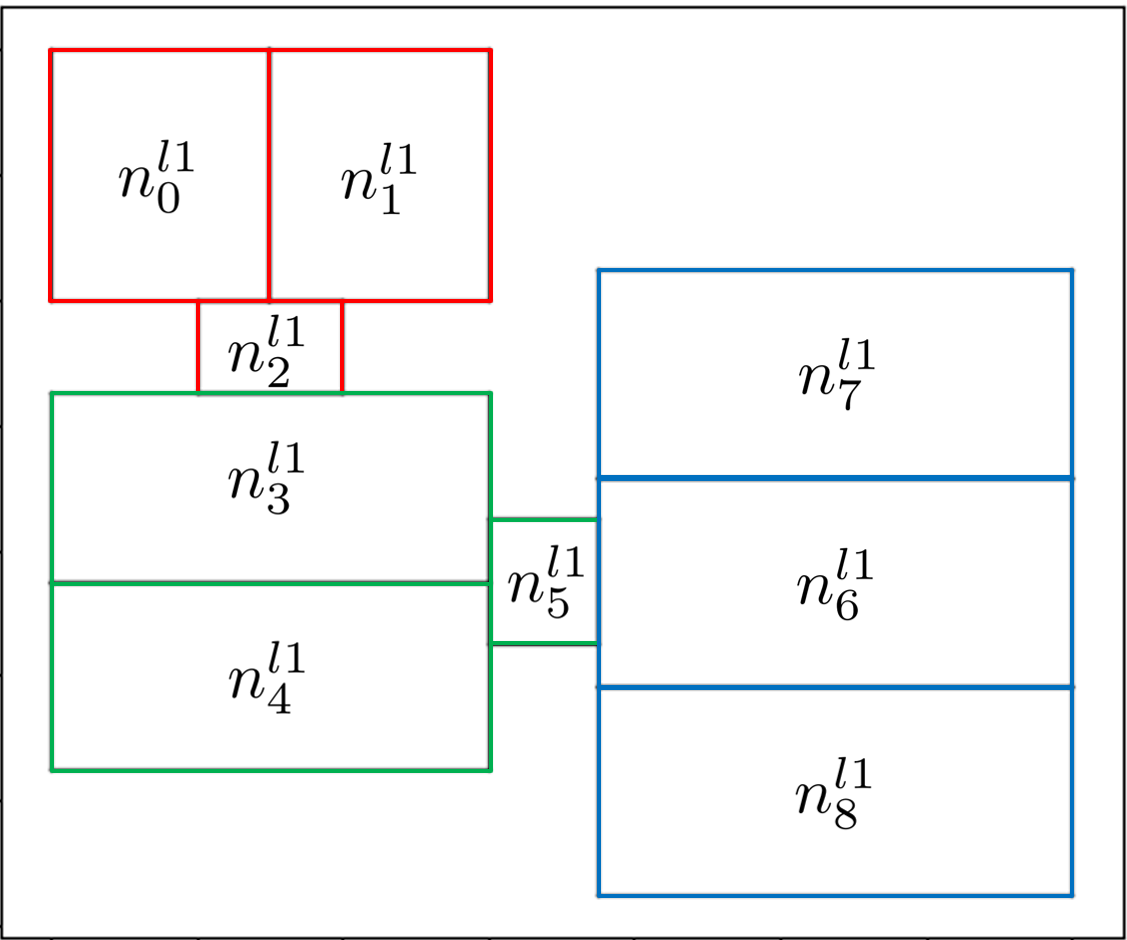
\includegraphics[width=\textwidth]{Report/images/layer1.png}
        \caption{Layer 1}
        \label{subfig:l1}
    \end{subfigure}
    \caption{A two layer framework for the three room environment. Each node in layer 0 corresponds to multiple nodes on layer 1. Layer 1 has the same discretisation as the original POMDP problem shown in Section \ref{fig:nodes}.}
    \label{fig:two_layers}
\end{figure}
The state, observation and action variables of layer 0 for the same environment are given by:
%
\begin{equation}\label{eq:l0}
    \begin{aligned}[t] 
        x_a^{l0} &\in \big\{n_0^{l0}, n_1^{l0}, n_2^{0}  \big\} \\
        x_k^{l0} &\in  \big\{n_0^{l0}, n_1^{l0}, n_2^{0}, \texttt{agent},\texttt{goal}  \big\}\\
        o_k^{l0} &\in \big\{\texttt{no}, n_0^{l0}, n_1^{l0}, n_2^{0}, \texttt{agent} \big\}\\
        a^{l0} &\in \begin{aligned}[t]\big\{&\texttt{nav($n_0^{l0}, n_1^{l0}$)}, \texttt{nav($n_1^{l0}, n_2^{l0}$)},\texttt{pickup}1, \ldots, \texttt{pickup}K, \texttt{release}\big\}.
        \end{aligned}
        %& & \cdots, \texttt{pickup}m, \texttt{release}\big\}
    \end{aligned}
\end{equation}
%
Because of the coarse discretisation not only is the state and observation space smaller but the action space is also smaller as fewer navigation actions are needed. Layer 1 corresponds to the original POMDP problem. The \texttt{look\_around} action exists only in the lowest layer POMDP:
%
\begin{equation}\label{eq:l1}
    \begin{aligned}[t] 
        x_a^{l1} &\in \big\{n_0^{l1}, \ldots, n_8^{l1} \big\} \\
        x_k^{l1} &\in  \big\{n_0^{l1},\ldots, n_8^{l1}, \texttt{agent},\texttt{goal}  \big\}\\
        o_k^{l1} &\in \big\{\texttt{no}, n_0^{l1},\ldots, n_8^{l1}, \texttt{agent} \big\}\\
        a^{l1} &\in \begin{aligned}[t]\big\{&\texttt{nav($n_0^{l0}, n_1^{l0}$)}, \ldots,\texttt{look\_around}, \texttt{pickup}1, \ldots, \texttt{pickup}K, \texttt{release}\big\}.
        \end{aligned}
        %& & \cdots, \texttt{pickup}m, \texttt{release}\big\}
    \end{aligned}
\end{equation}
For a larger environment more layers are needed to reach the desired discretisation level, such that each lowest layer node takes a few square meters. Each node in layer 1 is split into multiple non-overlapping subnodes. A large office environment with three layers of discretisation is shown in Figure \ref{fig:bigenv_3layers}. To achieve high speedups in computation time each node should be subdivided into 3-4 nodes as is further discussed in Section \ref{subsec:Multi-Scale_properties}.
%%%%%%%%%
\begin{figure}
    \centering
    \begin{subfigure}[b]{0.23\textwidth}
        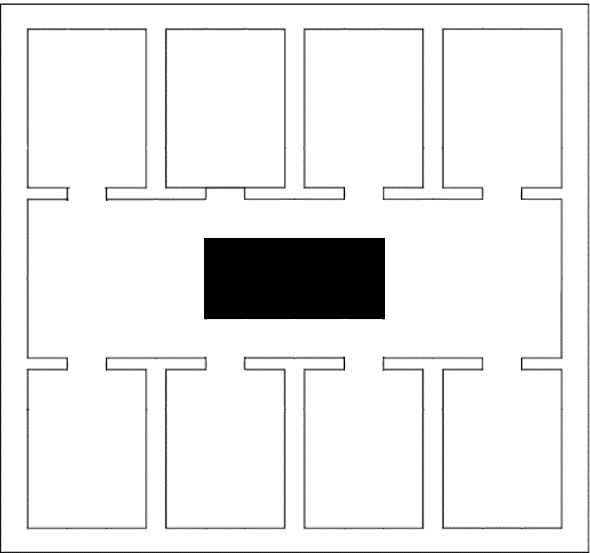
\includegraphics[width=\textwidth]{Report/images/Bilda.png}
        \caption[t]{Large office}
        \label{subfig:bigenv}
    \end{subfigure}
    \hfill
    \begin{subfigure}[b]{0.23\textwidth}
        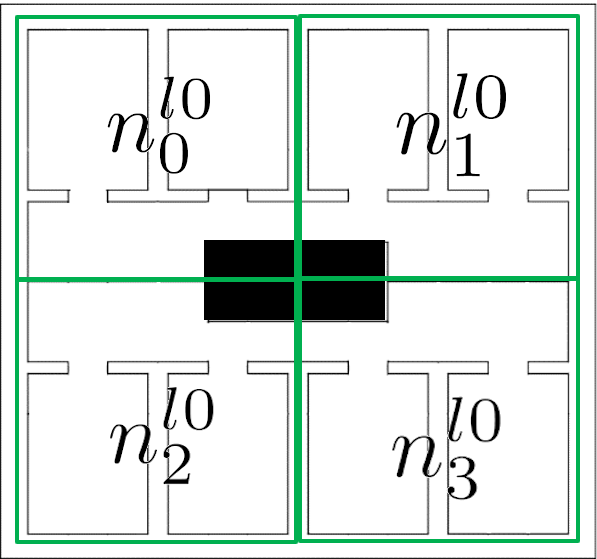
\includegraphics[width=\textwidth]{Report/images/Bildb_c.png}
        \caption{Layer 0}
        \label{subfig:bigenvl0}
    \end{subfigure}
     \hfill
    \begin{subfigure}[b]{0.23\textwidth}
        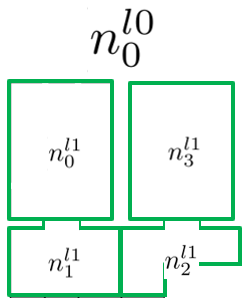
\includegraphics[width=0.85\textwidth]{Report/images/Bild1c.png}
        \caption{$n_0^{l0}$ on layer 1}
        \label{subfig:bigenvl1}
    \end{subfigure}
     \hfill
    \begin{subfigure}[b]{0.23\textwidth}
        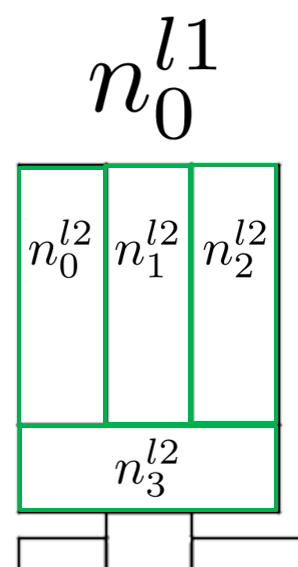
\includegraphics[width=0.6\textwidth]{Report/images/Bild1d.png}
        \caption{$n_0^{l1}$ on layer 2}
        \label{subfig:bigenvl2}
    \end{subfigure}
    \caption{Three layer discretisation of the large office environment.}
    \label{fig:bigenv_3layers}
\end{figure}
%%%%%%%%%%%%%%%%%%%%%%%%%%%%%
%%%%%%%%%%%%%%%%%%%%%%%%%%%
\subsubsection{Higher Layer Transition, Reward and Observation Model}
To solve the higher layers the respective transition, reward and observation models are needed. The lowest layer models are created as described in Section \ref{subsec:POMDPmodel}. The transition models of the higher layers can be formulated analogous to the lowest layer with Equations \ref{eq:Tnavxa}-\ref{eq:Txkts}. 
The higher layer reward and observation models are created from the lower layer ones in a recursive manner by using handcrafted open-loop policies. For each relevant state-action pair on layer $\lambda$ at least one open-loop policy $\pi_\text{OL}$ on layer $\lambda+1$ is required. The policy $\pi_\text{OL}$ is an ordered list where element $\pi_\text{OL}\texttt{[$i$]}$ is the $i$-th action to execute. The derivation of the higher layer reward model is first motivated by an example.
\begin{example}\label{ex:R_OL}
Consider the three room environment from Figure \ref{fig:two_layers}. The reward of layer 0 for the state where the agent starts in the first room and chooses the navigation action to drive to the second room needs to be computed. The open-loop policy on layer 1 that brings the agent from the first room to the second depends on the starting state on layer 1 and is shown in Equation \ref{eq:OL_example}:
\begin{equation}\label{eq:OL_example}
    \pi_\text{OL}(\texttt{nav($n_0^{l0}, n_1^{l0}$)}) = \begin{cases}
    \texttt{[nav($n_0^{l1}, n_2^{l1}$), nav($n_2^{l1}, n_3^{l1}$)]}, & \text{if starting state is }n_0^{l1};\\
    \texttt{[nav($n_1^{l1}, n_2^{l1}$), nav($n_2^{l1}, n_3^{l1}$)]}, & \text{if starting state is }n_1^{l1};\\
    \texttt{[nav($n_2^{l1}, n_3^{l1}$)]}, & \text{if starting state is }n_2^{l1}.
    \end{cases}
\end{equation}
The reward of executing $\pi_\text{OL}$ in $n_0^{l1}$ is calculated as the discounted summation of the rewards for each action:
\begin{equation}
    \begin{aligned}
    R^{\pi_\text{OL}}\left(x_a^{l1}=n_0^{l1}\right)=
    &R\left(x_a^{l1}=n_0^{l1}, a^{l1}=\texttt{nav($n_0^{l1}, n_2^{l1}$)} \right) \\
    &+ \gamma \cdot R\left(x_a^{l1}=n_2^{l1}, a^{l1}=\texttt{nav($n_2^{l1}, n_3^{l1}$)} \right).
\end{aligned}
\end{equation}
The layer 0 reward can now be calculated by averaging the reward of executing $\pi_\text{OL}$ for the different starting states:
\begin{equation}
    \begin{aligned}
       R\left(x_a^{l0}=n_0^{l0}, a^{l0}=\texttt{nav($n_0^{l0}, n_1^{l0}$)}\right) = \frac{1}{3}\cdot \big(&R^{\pi_\text{OL}}\left(x_a^{l1}=n_0^{l1}\right) + R^{\pi_\text{OL}}\left(x_a^{l1}=n_1^{l1}\right)\\
       &+ R^{\pi_\text{OL}}\left(x_a^{l1}=n_2^{l1}\right)\big).
    \end{aligned}
\end{equation}
Note that multiple open-loop policies could be used and the respective rewards averaged to the layer 0 reward. 
\demo
\end{example}

In a more general setup with a non-deterministic transition model the expected reward for following the open-loop policy $\pi_\text{OL}$ on layer $\lambda$ starting in state $s^{l\lambda}$ can be computed recursively as:
\begin{equation}\label{eq:R_OL}
    R^{\pi_\text{OL}}\left( s^{l\lambda} \right) = R\left(s^{l\lambda}, \pi_\text{OL}\texttt{[$1$]}\right) + \gamma \cdot \sum_{s'\in \mathcal{S}^{l\lambda}}T\left( s^{l\lambda}, a^{l\lambda}=\pi_\text{OL}\texttt{[$1$]}, s' \right)\cdot R^{\pi_\text{OL}\texttt{[$2$:]}}\left( s' \right)
\end{equation}
where $\pi_\text{OL}\texttt{[$2$:]}$ is the same list starting at the second element.\\
For the three layer hierarchy of Figure \ref{fig:bigenv_3layers} the models of layer 1 are created with the models of layer 2. The models of layer 0 can then be computed with the models of layer 1.\\

The higher layer observation models are constructed with the same approach. First, a mapping for the lower layer observations to the higher layer observation needs to be defined. One action of layer 0 corresponds to a policy on layer 1 which produces multiple observations. The observation of item $k$ in the higher layer takes the value $n_i$ if any of the observations on the lower layer is within $n_i$. If all observations on the lower layers are \texttt{no} the higher layer observation takes the value \texttt{no}:
\begin{equation}
    o_k^{l0} = \begin{cases}
    n_i^{l0}, &\text{if any }o_k^{l1}\in \SubNode(n_i^{l0});\\
    \texttt{no}, &\text{if all }o_k^{l1}=\texttt{no}.
    \end{cases}
\end{equation}
where $\SubNode(n_i^{l0})$ is the set of nodes on layer 1 that lie within $n_i^{l0}$. The higher layer observation model is again motivated by an example.
\begin{example}
Consider the three room environment and the open-loop policiy of Example \ref{ex:R_OL}. The probability of observing $o_k^{l0}=n_0^{l0}$ must be computed. The probability of observing the item in node $n_1^{l1}$ under $\pi_\text{OL}$ in start state $x_{a}^{l1}=n_0^{l1}$ is calculated as the probability of observing the item after the first action plus the probability of not observing the item in the first action but observing the item after any of the later actions:
\begin{equation}
    \begin{aligned}
        Z^{\pi_\text{OL}}\left( o_k^{l1}=n_1^{l1},x_{a}^{l1}=n_0^{l1} \right) = &Z\left(o^{l1}=n_1^{l1}, x_a^{l1\prime}=n_2^{l1}, a^{l1}=\texttt{nav($n_0^{l1}, n_2^{l1}$)} \right)\\
        &+ Z\left(o_k^{l1}=\texttt{no}, x_a^{l1\prime}=n_2^{l1}, a^{l1}=\texttt{nav($n_0^{l1}, n_2^{l1}$)} \right)\\
        &\cdot Z\left(o_k^{l1}=n_1^{l1}, x_a^{l1\prime}=n_3^{l1}, a^{l1}=\texttt{nav($n_2^{l1}, n_3^{l1}$)} \right).
    \end{aligned}
\end{equation}
The layer 0 observation model is calculated by averaging the observation model of executing $\pi_\text{OL}$ for the different starting states and the different observations that map to $n_0^{l0}$:
\begin{multline}
Z\left(o_k^{l0}=n_i^{l0},x_a^{l0\prime}=n_1^{l0}, a=\texttt{nav($n_0^{l0}, n_1^{l0}$)}\right) = \frac{1}{3}\bigg( \frac{1}{3}\sum_{o_k^{l1}\in\left\{n_0^{l1},n_1^{l1},n_2^{l1}\right\}} Z^{\pi_\text{OL}}\left( o_k^{l1},x_{a}^{l1\prime}=n_0^{l1} \right)\\
+\frac{1}{3}\sum_{o_k^{l1}\in\left\{n_0^{l1},n_1^{l1},n_2^{l1}\right\}} Z^{\pi_\text{OL}}\left( o_k^{l1},x_{a}^{l1\prime}=n_1^{l1} \right)     +\frac{1}{3}\sum_{o_k^{l1}\in\left\{n_0^{l1},n_1^{l1},n_2^{l1}\right\}} Z_k^{\pi_\text{OL}}\left( o_k^{l1},x_{a}^{l1\prime}=n_2^{l1} \right) \bigg).
\end{multline}
% \begin{equation}
%     \begin{aligned}
%         Z\left(o_k^{l0}=n_i^{l0},x_a{l0^\prime}=n_1^{l0}, a=\texttt{nav($n_0^{l0}, n_1^{l0}$)}\right) = \frac{1}{3}\bigg( &\frac{1}{3}\sum_{o_k^{l1}\in\left\{n_0^{l1},n_1^{l1},n_2^{l1}\right\}} Z^{\pi_\text{OL}}\left( o_k^{l1},x_{a,0}^{l1\prime}=n_0^{l1} \right)\\
%         &+\frac{1}{3}\sum_{o_k^{l1}\in\left\{n_0^{l1},n_1^{l1},n_2^{l1}\right\}} Z^{\pi_\text{OL}}\left( o_k^{l1},x_{a,0}^{l1\prime}=n_1^{l1} \right)  \\
%         & +\frac{1}{3}\sum_{o_k^{l1}\in\left\{n_0^{l1},n_1^{l1},n_2^{l1}\right\}} Z_k^{\pi_\text{OL}}\left( o_k^{l1},x_{a,0}^{l1\prime}=n_2^{l1} \right) \bigg).
%     \end{aligned}
% \end{equation}
The probability of not observing the item is one minus the probability of observing it:
\begin{multline}
    Z^{\pi_\text{OL}}\left( o_k^{l0}=\texttt{no}, x_a^{l0}=n_2^{l0}, a^{l0}=\texttt{nav($n_0^{l0},n_1^{l0}$)}\right) = \\
    1 - Z\left(o_k^{l0}=n_i^{l0},s'=n_1^{l0}, a=\texttt{nav($n_0^{l0}, n_1^{l0}$)}\right)
\end{multline}
\demo
\end{example}

For a more general setup the expected probability of observing item $k$ in $n_i^{l\lambda}$ under the open-loop policy $\pi_\text{OL}$ is computed recursively as:
\begin{equation}
    \begin{aligned}
        Z^{\pi_\text{OL}}\left( o^{l\lambda}=n_i^{l\lambda}, s_0^{l\lambda\prime}\right) = &\sum_{s'\in\mathcal{S}^{l\lambda}} T\left( s_0^{l\lambda}, \pi_\text{OL}\texttt{[$1$]}, s' \right) \cdot Z\left(o^{l\lambda}=n_i^{l\lambda}, s', \pi_\text{OL}\texttt{[$1$]}\right) \\
        &+ \gamma \cdot \sum_{s'\in\mathcal{S}^{l\lambda}} T\left( s_0^{l\lambda}, \pi_\text{OL}\texttt{[$1$]}, s' \right) \cdot O\left( o^{l\lambda}=\texttt{no}, s', \pi_\text{OL}\texttt{[$1$]} \right)\\
        &\cdot Z^{\pi_\text{OL}\texttt{[$2$:]}}\left( o^{l\lambda}=n_i^{l\lambda}, s_0^{l\lambda'} \right).
    \end{aligned}
\end{equation}

Instead of using open-loop policies one could also use closed-loop policies on states $\pi(s)$. This corresponds to the option/macro-action model for MDPs \cite{SUTTON1999181, DBLP:journals/corr/abs-1301-7381}. It is also possible to use automatically constructed closed-loop policies on beliefs \cite{7140035}.


%%%%%%%%%%%%%%%%%%%%%%%%%%%%%%%%%%%%%%%%%%%%%%%%%%%%%%%%%%%%%%%%%%%%%%%%%%%%%%%%%%%%%%%%%%%%%%%%%%%%%%%%%%%%%%%%
\subsection{Reasoning on Multiple Spatial Scales}\label{sec:M1toM3}
With the higher layer models it is now possible to solve each POMDP layer. In this subsection three different methods are shown on how the spatial layers can be combined. The methods differ in computation speed and lower layer reasoning ability. 
All methods consider a restricted state, action and observation space on the lower layers in order to get a speedup in computation time. 
%
\subsubsection{Method 01}\label{subsec:M1}
The first method explores a master-slave relationship between the layers where the lower layer tries to execute the action chosen by the layer above. The lower layers consider as few variables and values as strictly needed to execute the higher layer action. The transition, reward and observation model remain unchanged for the lower layers. To illustrate the concept an example of the restricted POMDP of layer 1 for each layer 0 action is given.
\begin{example}\label{ex:M1_nav}
Consider the three room environment from Figure \ref{fig:M1example} where the agent is currently in node $x_a^{l0}=n_0^{l0}$. Solving layer 0 yields the action $a^{l0}=\\ \texttt{nav($n_0^{l0},n_1^{l0}$)}$. The layer 1 POMDP only considers the nodes on layer 1 that are within the current layer 1 node $n_0^{l0}$ and the entry node to $n_1^{l0}$ which is $n_3^{l1}$. To navigate the agent, the items do not need to be considered in this sub-problem, which makes layer 1 an MDP. The terminal state on layer 0 is when the agent is within the node $n_1^{l0}$. The action space consists of navigation actions only:
\begin{equation}
     \begin{aligned}[t] 
        x_a^{l1} &\in \big\{n_0^{l1}, n_1^{l1}, n_2^{l1}, n_3^{l1}  \big\} \\
        s_t^{l1} &= \begin{pmatrix}x_a^{l1}=n_3^{l1} \end{pmatrix}^\intercal\\
        a^{l1} &\in \big\{\texttt{nav($n_0^{l1}, n_1^{l1}$)}, \texttt{nav($n_0^{l1}, n_2^{l1}$)}, \texttt{nav($n_1^{l1}, n_2^{l1}$)},\texttt{nav($n_2^{l1}, n_3^{l1}$)} \big\}.
    \end{aligned}
\end{equation}
\demo
\end{example}
\begin{figure}
    \centering
    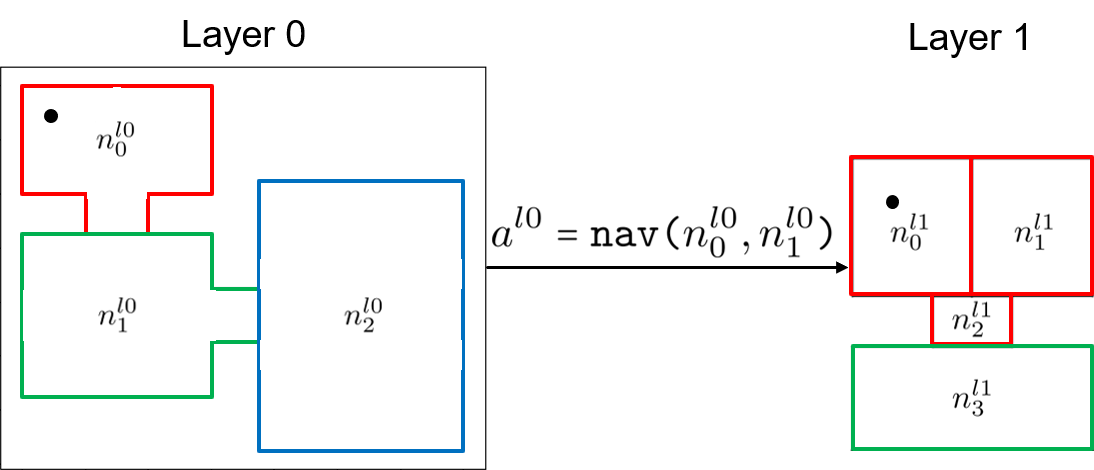
\includegraphics[width=\textwidth]{Report/images/exampleM1.png}
    \caption{Discretisation layers of Multi-Scale Method 01 in Example \ref{ex:M1_nav}. The black circle represents the agent's initial position.}
    \label{fig:M1example}
\end{figure}

\begin{example}
Consider the same scenario as in Example \ref{ex:M1_nav} but this time the agent is currently within $n_1^{l0}$ and the top layer action is a pickup action for the first item, i.e., $a^{l0}=\texttt{pickup}1$. On layer 1 the nodes considered are the ones within $n_1^{l0}$ and only the first item variable is necessary to perform the pickup action. The item variable can also take the value \texttt{not\_here} for which the initial belief is given as one minus the belief that the item is in $n_1^{l0}$. The action space contains the \texttt{look\_around} action which should be used to find the item within the current node. The terminal state is reached when the item is on the agent:
\begin{equation}
    \begin{aligned}[t] 
        x_a^{l1} &\in \big\{ n_3^{l1}, n_4^{l1}, n_5^{l1} \big\} \\
        x_1^{l1} &\in  \big\{ n_3^{l1}, n_4^{l1}, n_5^{l1}, \texttt{not\_here}, \texttt{agent} \big\}\\
         s_t^{l1} &= \begin{pmatrix} x_a^{l1} & x_1^{l1}=\texttt{agent} \end{pmatrix}^\intercal\\
        o_1^{l1} &\in \big\{\texttt{no},n_3^{l1}, n_4^{l1}, n_5^{l1}, \texttt{agent} \big\}\\
        a^{l1} &\in \big\{\texttt{nav($n_3^{l1}, n_4^{l1}$)}, \texttt{nav($n_3^{l1}, n_5^{l1}$)}, \texttt{nav($n_4^{l1}, n_5^{l1}$)}, \texttt{look\_around}, \texttt{pickup}1 \big\}.
        \end{aligned}
\end{equation}
 Note that the terminal state is unreachable if the item is not within $n_1^{l0}$. Since the POMDPs are solved in receding horizon fashion, i.e., layer 0 is solved again after the first action of layer 1 completes execution, this does not pose a problem.
 \demo
\end{example}

\begin{example}
In this example the agent is within $n_2^{l0}$ and carries the second item. Layer 0 chooses the \texttt{release} action. The terminal state in layer 1 is reached in any state where the item is not on the agent. The initial item value is observable and the transition model is deterministic. Thus the layer 1 sub-problem can be modelled as a MDP:
\begin{equation}
    \begin{aligned}[t] 
        x_a^{l1} &\in \big\{ n_6^{l1}, n_7^{l1}, n_8^{l1} \big\} \\
        x_2^{l1} &\in  \big\{ n_6^{l1}, n_7^{l1}, n_8^{l1}, \texttt{agent}, \texttt{goal} \big\}\\
        s_t^{l1} &= \begin{pmatrix} x_a & x_2\in\left\{ n_6^{l1}, n_7^{l1}, n_8^{l1}, \texttt{goal} \right\} \end{pmatrix}\\
        a^{l1} &\in \big\{\texttt{nav($n_6^{l1}, n_7^{l1}$)}, \texttt{nav($n_6^{l1}, n_8^{l1}$)}, \texttt{release} \big\}.
        \end{aligned}
\end{equation}
\demo
\end{example}
%
If layer $\lambda$ chooses a navigation action there can be an ambiguity on the layer $\lambda+1$ below if there are multiple terminal states within the same higher layer node. See Figure \ref{subfig:longroute} for a illustration. The agent is currently in node $n_1^{l2}$ and the terminal states are $n_4^{l2}$ and $n_6^{l2}$, both lie within the same node $n_1^{l1}$ on layer 1. Layer 2 will navigate to $n_4^{l2}$ since this minimizes the time to get to a terminal state. In the next time step the layer 1 POMDP will choose the \texttt{pickup}$1$ action to grab the item in node $n_6^{l2}$. Without further treatment the agent drives from the current node $n_1^{l2}$ to $n_4^{l6}$ and then to $n_6^{l2}$ instead of directly navigating from $n_1^{l2}$ to $n_6^{l2}$. \\

To get the desired behaviour shown in Figure \ref{subfig:shortroute} two POMDP problems on layer 2 need to be solved. First, layer 0 and layer 1 are solved to get the first action to execute. Then, the expected second action $a_\text{next}^{l1}$ on layer 1 is computed. In the situation depicted in Figure \ref{subfig:shortroute} $a_\text{next}^{l1}$ can directly be computed from the value function since $n_1^{l1}$ is not a terminal state on layer 1. Now the  POMDP on layer 2 for $a_\text{next}^{l1}$ is computed yielding the value function $V_\text{next}(b^{l2})$. Finally, the current layer 2 POMDP can be solved where the value function for the next POMDP problem is used as terminal state reward, i.e. the reward the agent receives for transitioning to a terminal state. In Equation \ref{eq:R_t_next} the terminal state reward for transitioning to node $n_4^{l2}$ assuming that the item is in node $n_6^{l2}$ is shown:
\begin{multline}\label{eq:R_t_next}
    R\big( s=\begin{pmatrix} x_a^{l2}=n_1^{l2} & x_1^{l2}=n_6^{l2} \end{pmatrix}^\intercal, a=\texttt{nav($n_1^{l2}, n_4^{l2}$)} \big) = \\
    V_\text{next}\big( x_a^{l2}=n_4^{l2}, b^{l2}(x_1^{l2}=n_6^{l2})=1 \big).
\end{multline}
Such a terminal state reward exists for all $x_a^{l2}, x_1^{l2}$ combinations. With the terminal state reward the agent now chooses the \texttt{nav($n_1^{l2}, n_6^{l2}$)} action as the value at node $n_6^{l2}$ is larger than in node $n_4^{l2}$. The described problem occurs for Method 02 and Method 03 as well and is solved with the same algorithmic solution.\\
\begin{figure}
    \centering
    \begin{subfigure}[b]{0.45\textwidth}
        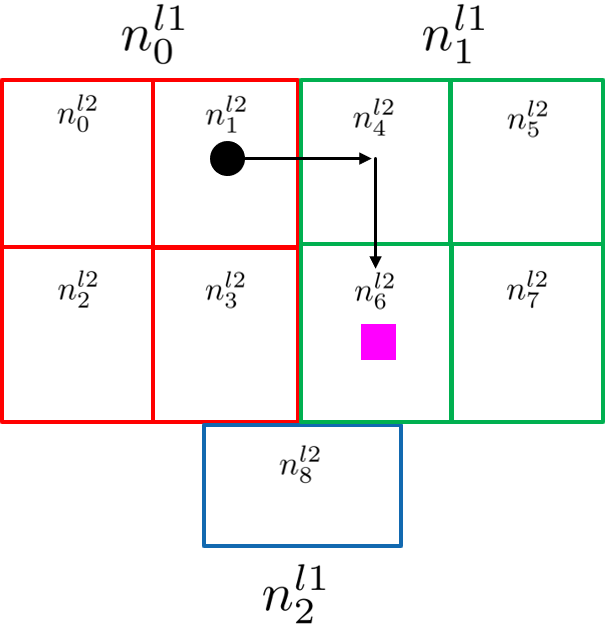
\includegraphics[width=\textwidth]{Report/images/two_terminal_states_longroute.png}
        \caption[t]{Solving one POMDP on layer 2}
        \label{subfig:longroute}
    \end{subfigure}
    \hfill
    \begin{subfigure}[b]{0.45\textwidth}
        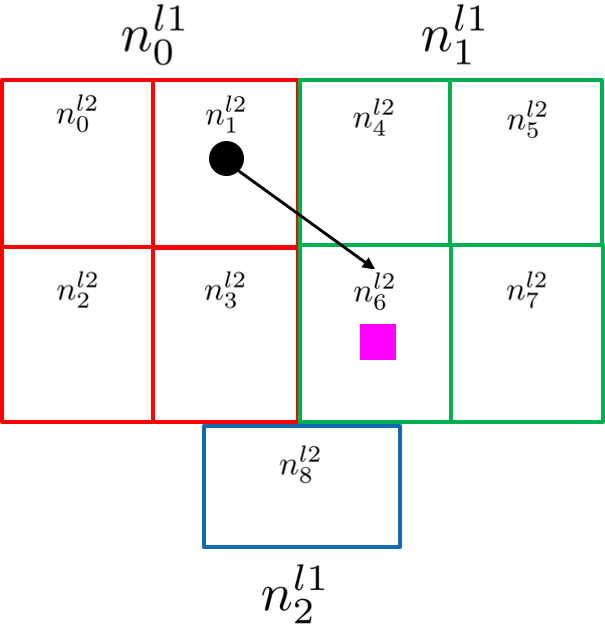
\includegraphics[width=\textwidth]{Report/images/two_terminal_states_shortroute.png}
        \caption{Solving two POMDPs on layer 2}
        \label{subfig:shortroute}
    \end{subfigure}
    \caption{Example situation where the layer 1 action $a^{l1}$ is \texttt{nav($n_0^{l1},n_1^{l1}$)}. The black dot represents the agent's start position and the pink square is the item location. In \ref{subfig:longroute} the agent's behaviour where only one POMDP is solved on layer 2 is shown and in \ref{subfig:shortroute} the same scenario when two layer 2 POMDPs are solved.}
    \label{fig:two_terminal_states}
\end{figure}

Method 01 yields a big speedup regarding computation time compared to solving the flat (single-layer) POMDP from Section \ref{subsec:POMDPmodel} as the state, action and observation space of both layer 0 and layer 1 is smaller. The drawback is that the lower layers perform very little reasoning and just try to solve the action of the layer above in as little time as possible. Since the higher layers use a coarse resolution their proposed action could be suboptimal. In Chapter \ref{sec:results} it is shown that such problems start to occur for larger environments where more than two layers are used. One particular problem for large environments is inconsistent search behaviour. The Method 01 agent stops the search in a room and goes to another room even though the belief that the item is in the room is still relatively high. See Section \ref{sec:cornercases} for a detailed example. 
The next two methods address those issues by giving the lower layers more flexibility and information about the entire problem.

%%%%%%%%%%%%%%%%%%%%%%%%%%%%%%%%%%%%%%%%%%%%%%%%%%%%%%%%%%%%%%%%%%%%%%%%%%%%%%%%%%%%%%%%%%%%%%%%%%%%%%%%%%%%%%%%
\subsubsection{Method 02}\label{subsec:M2}
The second method aims to improve the lower layer reasoning while still yielding a large computational speedup. The lower layers access the value function of the layer above to get global context about the problem. The value function can be incorporated through the terminal state reward as is shown in Example \ref{ex:M2_nav}. The lower layers can for example choose to explore the nodes before executing the proposed action of the layer above. This changes the belief at the terminal state and therefore the terminal state reward. Similarly as for Method 01, the state, action and observation space of the lower layers is determined by the higher layer state and action. However, all item variables are considered on all layers.

\begin{example}\label{ex:M2_nav}
Consider the same situation as in Example \ref{ex:M1_nav} and assume that the task involves two items. In contrast to Method 01, Method 02 considers both item variables on layer 1 and the action space contains the \texttt{look\_around} action:
\begin{equation}
    \begin{aligned}
         x_a^{l1} &\in \big\{n_0^{l1}, n_1^{l1}, n_2^{l1}, n_3^{l1}  \big\} \\
         x_1^{l1} &\in \big\{n_0^{l1}, n_1^{l1}, n_2^{l1}, n_3^{l1}, \texttt{not\_here} \big\} \ni x_2^{l1}\\
        s_t^{l1} &= \begin{pmatrix}x_a^{l1}=n_3^{l1} & x_1^{l1} & x_2^{l1} \end{pmatrix}^\intercal\\
        a^{l1} &\in \big\{\texttt{nav($n_0^{l1}, n_1^{l1}$)}, \texttt{nav($n_0^{l1}, n_2^{l1}$)}, \texttt{nav($n_1^{l1}, n_2^{l1}$)},\texttt{nav($n_2^{l1}, n_3^{l1}$)}, \texttt{look\_around)} \big\}.
    \end{aligned}
\end{equation}
This gives layer 1 the flexibility to search the first room before driving to the second room. The terminal state reward is an additional reward which is defined through the value function of layer 0. Note that there are 25 terminal states for all $x_1, x_2$ combinations, since both $x_1$ and $x_2$ take 5 different values . The terminal reward where the first item is in $n_1^{l1}$ and the second item in $n_3^{l1}$ is given by:  
\begin{multline}
    R_\text{terminal}\big(s^{l1}=\begin{pmatrix} x_a^{l1}=n_2^{l1} & x_1^{l1} = n_1^{l1} & x_2^{l1} = n_3^{l1} \end{pmatrix}^\intercal, a^{l1}=\texttt{nav($n_2^{l1},n_3^{l1}$)}\big)=\\
    V\big( x_a^{l0}=n_1^{l0}, b(x_1^{l0}=n_0^{l0})=1, b(x_2^{l0}=n_1^{l0})=1 \big).
\end{multline}
The belief vector $b^{l0}$ at the terminal state can be altered through the actions that the agent chooses. Through changing $b^{l0}$ the expected terminal reward changes (see Equation \ref{eq:R_b}), thus giving layer 1 context about the entire problem. 
\demo
\end{example}
The improved lower layer reasoning leads to better solutions as is shown in Chapter \ref{sec:results} but comes with the disadvantage of slightly longer computation times as all items are considered in the lower layers. Method 02 resolves the inconsistency problems of Method 01 as the lower layers tend to do more exploring. However, the lower layers still have to follow the proposed action of the above layers. This can become a problem for larger environments where the coarse discretisation of layer 0 can lead to suboptimal decisions. Method 03 resolves this limitation by adding additional terminal states to the lower layers.
%%%%%%%%%%%%%%%%%%%%%%%%%%%%%%%%%%%%%%%%%%%%%%%%%%%%%%%%%%%%%%%%%%%%%%%%%%%%%%%%%%%%%%%%%%%%%%%%%%%%%%%%%%%%%%%%
\subsubsection{Method 03}\label{subsec:M3}
The third method improves the lower layer reasoning by lifting the state restrictions coming from the proposed action of the above layer. The lower layer POMDPs are instead guided by the value function of the layer above which is incorporated as explained in Method 02. The concept is demonstrated in Example \ref{ex:M3}.

\begin{example}\label{ex:M3}
Consider a task with one item in the three room environment where the agent is currently in the second room, i.e. $x_a^{l0}=n_1^{l0}$. Solving layer 0 yields the value function $V(b^{l0})$. The restricted state, action and observation space is determined solely by the agent variable of layer 0. Terminal states are reached when the agent leaves the current room or if it successfully grabs an item:
\begin{equation}
    \begin{aligned}
        x_a^{l1} &\in \big\{ n_2^{l1}, n_3^{l1}, n_4^{l1}, n_5^{l1}, n_6^{l1} \big\} \\
        x_1^{l1} &\in  \big\{ n_2^{l1}, n_3^{l1}, n_4^{l1}, n_5^{l1}, n_6^{l1}, \texttt{not\_here}, \texttt{agent} \big\}\\
         s_t^{l1} &\in \big\{\begin{pmatrix} x_a^{l1}=n_2^{l1} & x_1^{l1} \end{pmatrix}^\intercal, \begin{pmatrix} x_a^{l1}=n_6^{l1} & x_1^{l1} \end{pmatrix}^\intercal,  \begin{pmatrix} x_a^{l1} & x_1^{l1}=\texttt{agent} \end{pmatrix}^\intercal \big\}\\
        o_1^{l1} &\in \big\{\texttt{no}, n_2^{l1}, n_3^{l1}, n_4^{l1}, n_5^{l1}, n_6^{l1}, \texttt{agent} \big\}\\
        a^{l1} &\in \big\{\texttt{nav($n_2^{l1}, n_3^{l1}$)}, \ldots,  \texttt{nav($n_5^{l1}, n_6^{l1}$)}, \texttt{look\_around}, \texttt{pickup}1 \big\}.
    \end{aligned}
\end{equation}
\demo
\end{example}
Layer 1 therefore has complete freedom in its action and does not need to follow the proposed action of layer 0 as was the case with Method 01 and Method 02. Through the better resolution of layer 1 the agent can sometimes correct for model approximation errors of layer 0. See Section \ref{sec:cornercases} for an example task in a large office environment where Method 03 performs a faster delivery than Method 01/02 because the lower layers choose a different path than layer 0 proposed. As one can see in the example, the state, action and observation space is larger than for Method 01/02 which increases computation time.\\

The current implementation of Method 03 comes with stability issues. In some situations the agent gets stuck navigating in between two nodes forever. The problem is illustrated in the made up scenario shown in Figure \ref{fig:stability}. The agent is currently in node $n_1^{l1}$ and the item is in $n_3^{l1}$ with belief 1 which makes this problem a MDP. Three terminal states are considered, one where the agent successfully  grabs the item and two at the layer 0 node $n_2^{l0}$:
\begin{equation}
    \begin{aligned}[t]
        s_{t,1} &= \begin{pmatrix}x_a^{l1} & x_1=\texttt{agent}\end{pmatrix}^\intercal \\
        s_{t,2} &= \begin{pmatrix}x_a^{l1}=n_9^{l1} & x_1\end{pmatrix}^\intercal\\
        s_{t,3} &= \begin{pmatrix}x_a^{l1}=n_{10}^{l1} & x_1\end{pmatrix}^\intercal
    \end{aligned}
\end{equation}
%
The terminal state reward for the first terminal state $s_{t,1}$ is given through the value function of layer 0 as:
\begin{equation}
    R_{\text{terminal,}1} = V\left(x_a^{l0}=n_0^{l0}, b(x_\text{mug}=\texttt{agent})=1\right).    
\end{equation}
The expected return under policy $\pi_1$ which navigates the agent to the item and picks it up is given by:
%
\begin{equation}
    \begin{aligned}
        V^{\pi_1} = &R_\text{time}(x_a=n_1^{l1}, a^{l1}=\texttt{nav($n_1^{l1}, n_2^{l1}$)})\\ 
        &+ \gamma\cdot R_\text{time}(x_a=n_2^{l1}, a^{l1}=\texttt{nav($n_2^{l1}, n_3^{l1}$)}) + \gamma^2 \cdot (R_\text{pickup} + R_{\text{terminal,}1}).
    \end{aligned}
\end{equation}
Similarly, the terminal state reward for the second terminal state $s_{t,2}$ is given by Equation \ref{eq:r_terminal2} and the value of following policy $\pi_2$ which brings the agent to the second terminal state is shown in Formula \ref{eq:Vpi2}:
\begin{equation}\label{eq:r_terminal2}
    R_{\text{terminal,}2} = V\left( x_a^{l0}=n_2^{l0}, b(x_\text{mug}=n_0^{l0})=1 \right)
\end{equation}
%
\begin{equation}\label{eq:Vpi2}
V^{\pi_2}=R_\text{time}\left( x_a^{l0}=n_1^{l1}, a=\texttt{nav($n_1^{l1}, n_9^{l1}$)} \right) + \gamma \cdot R_{\text{terminal,}2}.
\end{equation}
If $V^{\pi_2}$ is larger than $V^{\pi_1}$ the agent drives to node $n_9^{l1}$ instead of picking the item up. In the next move the agent will then drive back to node $n_1^{l1}$ as the item is within node $n_0^{l0}$. Thus, the initial situation is restored and the process starts over. The reason that $V^{\pi_2}$ could mistakenly be larger than $V^{\pi_1}$ is that $R_{\text{terminal},2}$ is given by the value function of layer 0. The value function at $x_a^{l0}=n_2^{l0}$ reflects that the agent is going to navigate from $n_2^{l0}$ to $n_0^{l2}$ in the next move and is then going to pick the item up. Layer 0 uses estimated reward functions created by averaging rewards of layer 1 as explained in Section \ref{subsec:Multi-Scale_overview}. Since the item is far away from the agent the actual value for picking the item up is smaller than layer 0 estimated. This makes the terminal state at $n_9^{l1}$ which can be reached with only small time penalty more attractive. In real scenarios such instability problems mostly occur if the problem has a broad belief distribution. For such cases the upper layer reward models are overconfident as they were created assuming simple open-loop policies.\\

The stability problems should be resolved by changing the way the higher layer reward and observation models are calculated. Instead of using open-loop policies a closed-loop policy $\pi_\text{CL}$ should be used. Consider the two-layer environment of Figure \ref{fig:two_layers}. The reward and observation model of the closed-loop policy is depending on the starting state $s^{l1}$. In the current implementation the layer 0 models are computed by averaging the models over all starting states in layer 1. Instead, the starting state resulting in the worst reward and observation probability must be used. This way, the layer 0 models are guaranteed to be overpessimistic. Layer 1 computes the optimal closed-loop policy $\pi^*\left(b^{l1}\right)$ which is by definition at least as good as $\pi_\text{CL}\left(b^{l1}\right)$. The value $V\left(b^{l0}\right)$ is therefore lower bound to $V(b^{l1})$, which resolves the stability issues. 


\begin{figure}
    \centering
    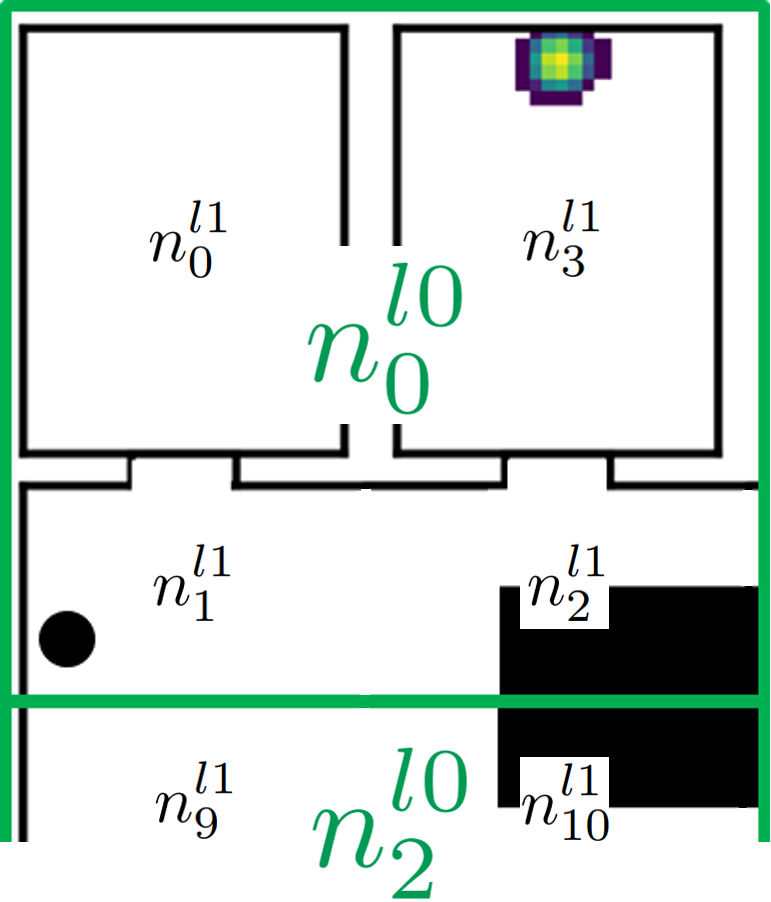
\includegraphics[width=0.4\textwidth]{Report/images/stability_2.png}
    \caption{Made-up scenario in a large office environment where the agent, represented as black circle, gets stuck driving in between node $n_1^{l1}$ and $n_9^{l1}$. The item is in $n_3^{l1}$ with belief one.}
    \label{fig:stability}
\end{figure}
%%%%%%%%%%%%%%%%%%%%%%%%%%%%%%%%%%%%%%%%%%%%%%%%%%%%%%%%%%%%%%%%%%%%%%%%%%%%%%%%%%%%%%%%%%%%%%%%%%%%%%%%%%%%%%%%

\subsection{Properties}\label{subsec:Multi-Scale_properties}
A qualitative comparison of some of the properties of the different Multi-Scale methods and the flat POMDP agent (Section \ref{sec:POMDPagent}) are summarized in Table \ref{tab:properties}.  The Multi-Scale methods split one large POMDP into multiple smaller POMDPs. With the hierarchical layout from Figure \ref{fig:bigenv_3layers}, where each node in is split into 4 subnodes on the next lower layer, a logarithmic relationship between the number of nodes in the flat problem and the number of layers in the hierarchy is given:
\begin{equation}
    N_\text{layers} \sim \log_4 N_\text{nodes}.
\end{equation}
This is a nice scaling property as the number of layers is proportional\footnote{As explained in Section \ref{sec:M1toM3} there are cases where multiple POMDP problems need to be solved on one layer.} to the number of POMDP problems that must be solved. \\

\begin{table}[h]
    \centering
    \begin{tabular}{l c c c c}
    \toprule
         &  M1 & M2 & M3 & Flat\\
    \midrule
        \addlinespace
         comp. speed & $+++$ & $++$ & $+$ & $---$ \\
         \addlinespace
         consistency & $-$ & $+$ & $+$ & $+++$ \\
         \addlinespace
         lower layer reasoning & $-$ & $+$ & $++$ & $+++$ \\
         \addlinespace
         stability issues & no & no& yes & no\\
         \addlinespace
    \bottomrule
    \end{tabular}
    \caption{Qualitative comparison of the different POMDP agents.}
    \label{tab:properties}
\end{table}
In general, all Multi-Scale methods create suboptimal solutions due to discretisation inaccuracies. A demonstration is depicted in Figure \ref{fig:suboptimal} where the task involves two items in the three room environment. Both items are within the same layer 0 node $n_0^{l0}$ and both goal-locations are in $n_2^{l0}$. Layer 0 is unable to differentiate the two items regarding expected delivery time and randomly chooses either the \texttt{pickup}1 or \texttt{pickup}2 action first. Layer 1 is guided through the layer 0 action $a^{l0}$ and value function $V(b^{l0})$. Neither reflects that the pink item's goal location is closer and should therefore be delivered first. The Multi-Scale agents can therefore not correctly reason which item to deliver first. The flat POMDP delivers the pink item first as the initial positions and goal locations of the two items are in different nodes. 
\begin{figure}[h]
    \centering
    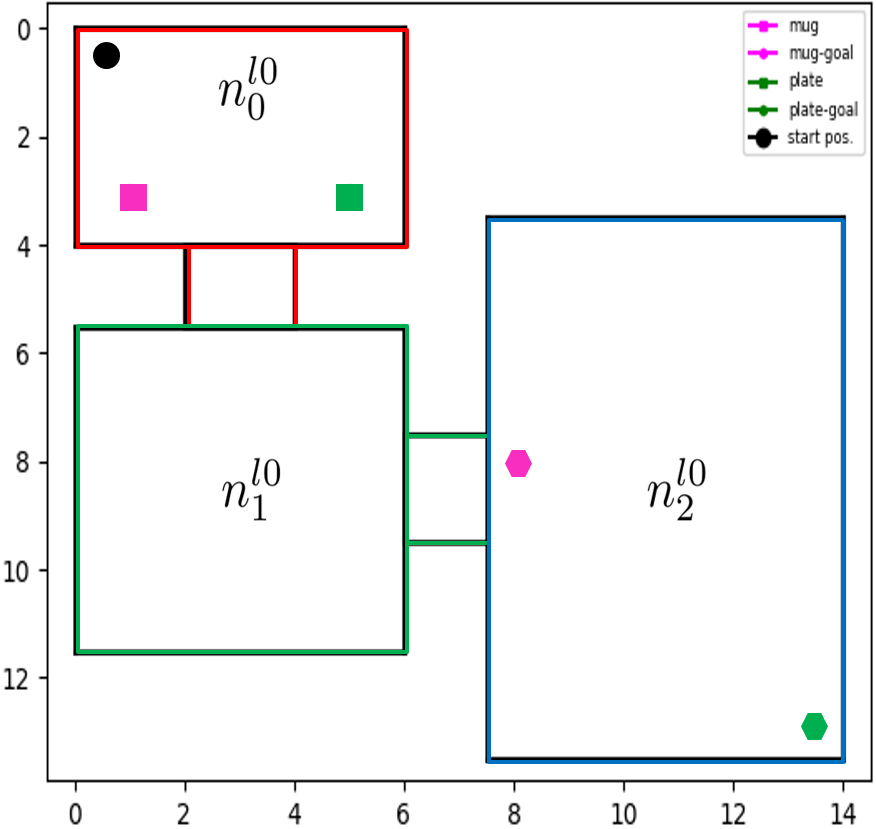
\includegraphics[width=0.5\textwidth]{Report/images/suboptimal.png}
    \caption{A scenario where the Multi-Scale methods are not able to correctly reason which item should be delivered first.}
    \label{fig:suboptimal}
\end{figure}
